%%%%%%%%%%%%%%%%%%%%%%%%%%%%%%%%%%%%%%%%%
% The Legrand Orange Book
% LaTeX Template
% Version 2.0 (9/2/15)
%
% This template has been downloaded from:
% http://www.LaTeXTemplates.com
%
% Mathias Legrand (legrand.mathias@gmail.com) with modifications by:
% Vel (vel@latextemplates.com)
%
% License:
% CC BY-NC-SA 3.0 (http://creativecommons.org/licenses/by-nc-sa/3.0/)
%
% Compiling this template:
% This template uses biber for its bibliography and makeindex for its index.
% When you first open the template, compile it from the command line with the 
% commands below to make sure your LaTeX distribution is configured correctly:
%
% 1) pdflatex main
% 2) makeindex main.idx -s StyleInd.ist
% 3) biber main
% 4) pdflatex main x 2
%
% After this, when you wish to update the bibliography/index use the appropriate
% command above and make sure to compile with pdflatex several times 
% afterwards to propagate your changes to the document.
%
% This template also uses a number of packages which may need to be
% updated to the newest versions for the template to compile. It is strongly
% recommended you update your LaTeX distribution if you have any
% compilation errors.
%
% Important note:
% Chapter heading images should have a 2:1 width:height ratio,
% e.g. 920px width and 460px height.
%
%%%%%%%%%%%%%%%%%%%%%%%%%%%%%%%%%%%%%%%%%

%----------------------------------------------------------------------------------------
%	PACKAGES AND OTHER DOCUMENT CONFIGURATIONS
%----------------------------------------------------------------------------------------

\documentclass[11pt,fleqn]{book} % Default font size and left-justified equations

%----------------------------------------------------------------------------------------
\usepackage{bbold}%% $\mathbb{abc}$

%%%%%%%%%%%%%%%%%%%%%%%%%%%%%%%%%%%%%%%%%
% The Legrand Orange Book
% Structural Definitions File
% Version 2.0 (9/2/15)
%
% Original author:
% Mathias Legrand (legrand.mathias@gmail.com) with modifications by:
% Vel (vel@latextemplates.com)
% 
% This file has been downloaded from:
% http://www.LaTeXTemplates.com
%
% License:
% CC BY-NC-SA 3.0 (http://creativecommons.org/licenses/by-nc-sa/3.0/)
%
%%%%%%%%%%%%%%%%%%%%%%%%%%%%%%%%%%%%%%%%%

%----------------------------------------------------------------------------------------
%	VARIOUS REQUIRED PACKAGES AND CONFIGURATIONS
%----------------------------------------------------------------------------------------

\usepackage[top=3cm,bottom=3cm,left=3cm,right=3cm,headsep=10pt,a4paper]{geometry} % Page margins

\usepackage{graphicx} % Required for including pictures
\graphicspath{{Pictures/}} % Specifies the directory where pictures are stored

\usepackage{lipsum} % Inserts dummy text

\usepackage{tikz} % Required for drawing custom shapes

\usepackage[english]{babel} % English language/hyphenation

\usepackage{enumitem} % Customize lists
\setlist{nolistsep} % Reduce spacing between bullet points and numbered lists

\usepackage{booktabs} % Required for nicer horizontal rules in tables

\usepackage{xcolor} % Required for specifying colors by name
%\definecolor{ocre}{RGB}{243,102,25} % Define the orange color used for highlighting throughout the book
\definecolor{ocre}{RGB}{16,81,15} % Define the orange color used for highlighting throughout the book

%----------------------------------------------------------------------------------------
%	FONTS
%----------------------------------------------------------------------------------------

\usepackage{avant} % Use the Avantgarde font for headings
%\usepackage{times} % Use the Times font for headings
\usepackage{mathptmx} % Use the Adobe Times Roman as the default text font together with math symbols from the Sym­bol, Chancery and Com­puter Modern fonts

\usepackage{microtype} % Slightly tweak font spacing for aesthetics
\usepackage[utf8]{inputenc} % Required for including letters with accents
\usepackage[T1]{fontenc} % Use 8-bit encoding that has 256 glyphs

%----------------------------------------------------------------------------------------
%	BIBLIOGRAPHY AND INDEX
%----------------------------------------------------------------------------------------

\usepackage[style=numeric,citestyle=numeric,sorting=nyt,sortcites=true,autopunct=true,babel=hyphen,hyperref=true,abbreviate=false,backref=true,backend=biber]{biblatex}
\addbibresource{bibliography.bib} % BibTeX bibliography file
\defbibheading{bibempty}{}

\usepackage{calc} % For simpler calculation - used for spacing the index letter headings correctly
\usepackage{makeidx} % Required to make an index
\makeindex % Tells LaTeX to create the files required for indexing

%----------------------------------------------------------------------------------------
%	MAIN TABLE OF CONTENTS
%----------------------------------------------------------------------------------------

\usepackage{titletoc} % Required for manipulating the table of contents

\contentsmargin{0cm} % Removes the default margin

% Part text styling
\titlecontents{part}[0cm]
{\addvspace{20pt}\centering\large\bfseries}
{}
{}
{}

% Chapter text styling
\titlecontents{chapter}[1.25cm] % Indentation
{\addvspace{12pt}\large\sffamily\bfseries} % Spacing and font options for chapters
{\color{ocre!60}\contentslabel[\Large\thecontentslabel]{1.25cm}\color{ocre}} % Chapter number
{\color{ocre}}  
{\color{ocre!60}\normalsize\;\titlerule*[.5pc]{.}\;\thecontentspage} % Page number

% Section text styling
\titlecontents{section}[1.25cm] % Indentation
{\addvspace{3pt}\sffamily\bfseries} % Spacing and font options for sections
{\contentslabel[\thecontentslabel]{1.25cm}} % Section number
{}
{\hfill\color{black}\thecontentspage} % Page number
[]

% Subsection text styling
\titlecontents{subsection}[1.25cm] % Indentation
{\addvspace{1pt}\sffamily\small} % Spacing and font options for subsections
{\contentslabel[\thecontentslabel]{1.25cm}} % Subsection number
{}
{\ \titlerule*[.5pc]{.}\;\thecontentspage} % Page number
[]

% List of figures
\titlecontents{figure}[0em]
{\addvspace{-5pt}\sffamily}
{\thecontentslabel\hspace*{1em}}
{}
{\ \titlerule*[.5pc]{.}\;\thecontentspage}
[]

% List of tables
\titlecontents{table}[0em]
{\addvspace{-5pt}\sffamily}
{\thecontentslabel\hspace*{1em}}
{}
{\ \titlerule*[.5pc]{.}\;\thecontentspage}
[]

%----------------------------------------------------------------------------------------
%	MINI TABLE OF CONTENTS IN PART HEADS
%----------------------------------------------------------------------------------------

% Chapter text styling
\titlecontents{lchapter}[0em] % Indenting
{\addvspace{15pt}\large\sffamily\bfseries} % Spacing and font options for chapters
{\color{ocre}\contentslabel[\Large\thecontentslabel]{1.25cm}\color{ocre}} % Chapter number
{}  
{\color{ocre}\normalsize\sffamily\bfseries\;\titlerule*[.5pc]{.}\;\thecontentspage} % Page number

% Section text styling
\titlecontents{lsection}[0em] % Indenting
{\sffamily\small} % Spacing and font options for sections
{\contentslabel[\thecontentslabel]{1.25cm}} % Section number
{}
{}

% Subsection text styling
\titlecontents{lsubsection}[.5em] % Indentation
{\normalfont\footnotesize\sffamily} % Font settings
{}
{}
{}

%----------------------------------------------------------------------------------------
%	PAGE HEADERS
%----------------------------------------------------------------------------------------

\usepackage{fancyhdr} % Required for header and footer configuration

\pagestyle{fancy}
\renewcommand{\chaptermark}[1]{\markboth{\sffamily\normalsize\bfseries\chaptername\ \thechapter.\ #1}{}} % Chapter text font settings
\renewcommand{\sectionmark}[1]{\markright{\sffamily\normalsize\thesection\hspace{5pt}#1}{}} % Section text font settings
\fancyhf{} \fancyhead[LE,RO]{\sffamily\normalsize\thepage} % Font setting for the page number in the header
\fancyhead[LO]{\rightmark} % Print the nearest section name on the left side of odd pages
\fancyhead[RE]{\leftmark} % Print the current chapter name on the right side of even pages
\renewcommand{\headrulewidth}{0.5pt} % Width of the rule under the header
\addtolength{\headheight}{2.5pt} % Increase the spacing around the header slightly
\renewcommand{\footrulewidth}{0pt} % Removes the rule in the footer
\fancypagestyle{plain}{\fancyhead{}\renewcommand{\headrulewidth}{0pt}} % Style for when a plain pagestyle is specified

% Removes the header from odd empty pages at the end of chapters
\makeatletter
\renewcommand{\cleardoublepage}{
\clearpage\ifodd\c@page\else
\hbox{}
\vspace*{\fill}
\thispagestyle{empty}
\newpage
\fi}

%----------------------------------------------------------------------------------------
%	THEOREM STYLES
%----------------------------------------------------------------------------------------

\usepackage{amsmath,amsfonts,amssymb,amsthm} % For math equations, theorems, symbols, etc

\newcommand{\intoo}[2]{\mathopen{]}#1\,;#2\mathclose{[}}
\newcommand{\ud}{\mathop{\mathrm{{}d}}\mathopen{}}
\newcommand{\intff}[2]{\mathopen{[}#1\,;#2\mathclose{]}}
\newtheorem{notation}{Notação}[chapter]

% Boxed/framed environments
\newtheoremstyle{ocrenumbox}% % Theorem style name
{0pt}% Space above
{0pt}% Space below
{\normalfont}% % Body font
{}% Indent amount
{\small\bf\sffamily\color{ocre}}% % Theorem head font
{\;}% Punctuation after theorem head
{0.25em}% Space after theorem head
{\small\sffamily\color{ocre}\thmname{#1}\nobreakspace\thmnumber{\@ifnotempty{#1}{}\@upn{#2}}% Theorem text (e.g. Theorem 2.1)
\thmnote{\nobreakspace\the\thm@notefont\sffamily\bfseries\color{black}---\nobreakspace#3.}} % Optional theorem note
\renewcommand{\qedsymbol}{$\blacksquare$}% Optional qed square

\newtheoremstyle{blacknumex}% Theorem style name
{5pt}% Space above
{5pt}% Space below
{\normalfont}% Body font
{} % Indent amount
{\small\bf\sffamily}% Theorem head font
{\;}% Punctuation after theorem head
{0.25em}% Space after theorem head
{\small\sffamily{\tiny\ensuremath{\blacksquare}}\nobreakspace\thmname{#1}\nobreakspace\thmnumber{\@ifnotempty{#1}{}\@upn{#2}}% Theorem text (e.g. Theorem 2.1)
\thmnote{\nobreakspace\the\thm@notefont\sffamily\bfseries---\nobreakspace#3.}}% Optional theorem note

\newtheoremstyle{blacknumbox} % Theorem style name
{0pt}% Space above
{0pt}% Space below
{\normalfont}% Body font
{}% Indent amount
{\small\bf\sffamily}% Theorem head font
{\;}% Punctuation after theorem head
{0.25em}% Space after theorem head
{\small\sffamily\thmname{#1}\nobreakspace\thmnumber{\@ifnotempty{#1}{}\@upn{#2}}% Theorem text (e.g. Theorem 2.1)
\thmnote{\nobreakspace\the\thm@notefont\sffamily\bfseries---\nobreakspace#3.}}% Optional theorem note

% Non-boxed/non-framed environments
\newtheoremstyle{ocrenum}% % Theorem style name
{5pt}% Space above
{5pt}% Space below
{\normalfont}% % Body font
{}% Indent amount
{\small\bf\sffamily\color{ocre}}% % Theorem head font
{\;}% Punctuation after theorem head
{0.25em}% Space after theorem head
{\small\sffamily\color{ocre}\thmname{#1}\nobreakspace\thmnumber{\@ifnotempty{#1}{}\@upn{#2}}% Theorem text (e.g. Theorem 2.1)
\thmnote{\nobreakspace\the\thm@notefont\sffamily\bfseries\color{black}---\nobreakspace#3.}} % Optional theorem note
\renewcommand{\qedsymbol}{$\blacksquare$}% Optional qed square
\makeatother

% Defines the theorem text style for each type of theorem to one of the three styles above
\newcounter{dummy} 
\numberwithin{dummy}{section}
\theoremstyle{ocrenumbox}
\newtheorem{theoremeT}[dummy]{Teorema}
\newtheorem{problemT}{Problema}[chapter]
\newtheorem{exerciseT}{Exercise}[chapter]
\theoremstyle{blacknumex}
\newtheorem{exampleT}{Example}[chapter]
\theoremstyle{blacknumbox}
\newtheorem{vocabulary}{Vocabulary}[chapter]
\newtheorem{definitionT}{Definição}[section]
\newtheorem{corollaryT}[dummy]{Corolário}
\newtheorem{myproofT}{Prova} [chapter]
\theoremstyle{ocrenum}
\newtheorem{propositionT}[dummy]{Proposição}

%----------------------------------------------------------------------------------------
%	DEFINITION OF COLORED BOXES
%----------------------------------------------------------------------------------------

\RequirePackage[framemethod=default]{mdframed} % Required for creating the theorem, definition, exercise and corollary boxes

% Theorem box
\newmdenv[skipabove=7pt,
skipbelow=7pt,
backgroundcolor=black!5,
linecolor=ocre,
innerleftmargin=5pt,
innerrightmargin=5pt,
innertopmargin=5pt,
leftmargin=0cm,
rightmargin=0cm,
innerbottommargin=5pt]{tBox}

% Proposition box
\newmdenv[skipabove=7pt,
skipbelow=7pt,
backgroundcolor=blue!5,
linecolor=ocre,
innerleftmargin=5pt,
innerrightmargin=5pt,
innertopmargin=5pt,
leftmargin=0cm,
rightmargin=0cm,
innerbottommargin=5pt]{ppBox}

% Exercise box	  
\newmdenv[skipabove=7pt,
skipbelow=7pt,
rightline=false,
leftline=true,
topline=false,
bottomline=false,
backgroundcolor=ocre!10,
linecolor=ocre,
innerleftmargin=5pt,
innerrightmargin=5pt,
innertopmargin=5pt,
innerbottommargin=5pt,
leftmargin=0cm,
rightmargin=0cm,
linewidth=4pt]{eBox}	


% Problem box	  
\newmdenv[skipabove=7pt,
skipbelow=7pt,
rightline=false,
leftline=true,
topline=false,
bottomline=false,
backgroundcolor=ocre!10,
linecolor=ocre,
innerleftmargin=5pt,
innerrightmargin=5pt,
innertopmargin=5pt,
innerbottommargin=5pt,
leftmargin=0cm,
rightmargin=0cm,
linewidth=4pt]{pBox}	

% Definition box
\newmdenv[skipabove=7pt,
skipbelow=7pt,
rightline=false,
leftline=true,
topline=false,
bottomline=false,
linecolor=ocre,
innerleftmargin=5pt,
innerrightmargin=5pt,
innertopmargin=0pt,
leftmargin=0cm,
rightmargin=0cm,
linewidth=4pt,
innerbottommargin=0pt]{dBox}	

% Corollary box
\newmdenv[skipabove=7pt,
skipbelow=7pt,
rightline=false,
leftline=true,
topline=false,
bottomline=false,
linecolor=gray,
backgroundcolor=black!5,
innerleftmargin=5pt,
innerrightmargin=5pt,
innertopmargin=5pt,
leftmargin=0cm,
rightmargin=0cm,
linewidth=4pt,
innerbottommargin=5pt]{cBox}

% Creates an environment for each type of theorem and assigns it a theorem text style from the "Theorem Styles" section above and a colored box from above
\newenvironment{theorem}{\begin{tBox}\begin{theoremeT}}{\end{theoremeT}\end{tBox}}
\newenvironment{proposition}{\begin{ppBox}\begin{propositionT}}{\end{propositionT}\end{ppBox}}
\newenvironment{exercise}{\begin{eBox}\begin{exerciseT}}{\hfill{\color{ocre}\tiny\ensuremath{\blacksquare}}\end{exerciseT}\end{eBox}}			
\newenvironment{problem}{\begin{pBox}\begin{problemT}}{\hfill{\color{ocre}\tiny\ensuremath{\blacksquare}}\end{problemT}\end{pBox}}				  
\newenvironment{definition}{\begin{dBox}\begin{definitionT}}{\end{definitionT}\end{dBox}}	
\newenvironment{example}{\begin{exampleT}}{\hfill{\tiny\ensuremath{\blacksquare}}\end{exampleT}}		
\newenvironment{corollary}{\begin{cBox}\begin{corollaryT}}{\end{corollaryT}\end{cBox}}	

%----------------------------------------------------------------------------------------
%	REMARK ENVIRONMENT
%----------------------------------------------------------------------------------------

\newenvironment{remark}{\par\vspace{10pt}\small % Vertical white space above the remark and smaller font size
\begin{list}{}{
\leftmargin=35pt % Indentation on the left
\rightmargin=25pt}\item\ignorespaces % Indentation on the right
\makebox[-2.5pt]{\begin{tikzpicture}[overlay]
\node[draw=ocre!60,line width=1pt,circle,fill=ocre!25,font=\sffamily\bfseries,inner sep=2pt,outer sep=0pt] at (-15pt,0pt){\textcolor{ocre}{R}};\end{tikzpicture}} % Orange R in a circle
\advance\baselineskip -1pt}{\end{list}\vskip5pt} % Tighter line spacing and white space after remark

%----------------------------------------------------------------------------------------
%	SECTION NUMBERING IN THE MARGIN
%----------------------------------------------------------------------------------------

\makeatletter
\renewcommand{\@seccntformat}[1]{\llap{\textcolor{ocre}{\csname the#1\endcsname}\hspace{1em}}}                    
\renewcommand{\section}{\@startsection{section}{1}{\z@}
{-4ex \@plus -1ex \@minus -.4ex}
{1ex \@plus.2ex }
{\normalfont\large\sffamily\bfseries}}
\renewcommand{\subsection}{\@startsection {subsection}{2}{\z@}
{-3ex \@plus -0.1ex \@minus -.4ex}
{0.5ex \@plus.2ex }
{\normalfont\sffamily\bfseries}}
\renewcommand{\subsubsection}{\@startsection {subsubsection}{3}{\z@}
{-2ex \@plus -0.1ex \@minus -.2ex}
{.2ex \@plus.2ex }
{\normalfont\small\sffamily\bfseries}}                        
\renewcommand\paragraph{\@startsection{paragraph}{4}{\z@}
{-2ex \@plus-.2ex \@minus .2ex}
{.1ex}
{\normalfont\small\sffamily\bfseries}}

%----------------------------------------------------------------------------------------
%	PART HEADINGS
%----------------------------------------------------------------------------------------

% numbered part in the table of contents
\newcommand{\@mypartnumtocformat}[2]{%
\setlength\fboxsep{0pt}%
\noindent\colorbox{ocre!20}{\strut\parbox[c][.7cm]{\ecart}{\color{ocre!70}\Large\sffamily\bfseries\centering#1}}\hskip\esp\colorbox{ocre!40}{\strut\parbox[c][.7cm]{\linewidth-\ecart-\esp}{\Large\sffamily\centering#2}}}%
%%%%%%%%%%%%%%%%%%%%%%%%%%%%%%%%%%
% unnumbered part in the table of contents
\newcommand{\@myparttocformat}[1]{%
\setlength\fboxsep{0pt}%
\noindent\colorbox{ocre!40}{\strut\parbox[c][.7cm]{\linewidth}{\Large\sffamily\centering#1}}}%
%%%%%%%%%%%%%%%%%%%%%%%%%%%%%%%%%%
\newlength\esp
\setlength\esp{4pt}
\newlength\ecart
\setlength\ecart{1.2cm-\esp}
\newcommand{\thepartimage}{}%
\newcommand{\partimage}[1]{\renewcommand{\thepartimage}{#1}}%
\def\@part[#1]#2{%
\ifnum \c@secnumdepth >-2\relax%
\refstepcounter{part}%
\addcontentsline{toc}{part}{\texorpdfstring{\protect\@mypartnumtocformat{\thepart}{#1}}{\partname~\thepart\ ---\ #1}}
\else%
\addcontentsline{toc}{part}{\texorpdfstring{\protect\@myparttocformat{#1}}{#1}}%
\fi%
\startcontents%
\markboth{}{}%
{\thispagestyle{empty}%
\begin{tikzpicture}[remember picture,overlay]%
\node at (current page.north west){\begin{tikzpicture}[remember picture,overlay]%	
\fill[ocre!20](0cm,0cm) rectangle (\paperwidth,-\paperheight);
\node[anchor=north] at (4cm,-3.25cm){\color{ocre!40}\fontsize{220}{100}\sffamily\bfseries\@Roman\c@part}; 
\node[anchor=south east] at (\paperwidth-1cm,-\paperheight+1cm){\parbox[t][][t]{8.5cm}{
\printcontents{l}{0}{\setcounter{tocdepth}{1}}%
}};
\node[anchor=north east] at (\paperwidth-1.5cm,-3.25cm){\parbox[t][][t]{15cm}{\strut\raggedleft\color{white}\fontsize{30}{30}\sffamily\bfseries#2}};
\end{tikzpicture}};
\end{tikzpicture}}%
\@endpart}
\def\@spart#1{%
\startcontents%
\phantomsection
{\thispagestyle{empty}%
\begin{tikzpicture}[remember picture,overlay]%
\node at (current page.north west){\begin{tikzpicture}[remember picture,overlay]%	
\fill[ocre!20](0cm,0cm) rectangle (\paperwidth,-\paperheight);
\node[anchor=north east] at (\paperwidth-1.5cm,-3.25cm){\parbox[t][][t]{15cm}{\strut\raggedleft\color{white}\fontsize{30}{30}\sffamily\bfseries#1}};
\end{tikzpicture}};
\end{tikzpicture}}
\addcontentsline{toc}{part}{\texorpdfstring{%
\setlength\fboxsep{0pt}%
\noindent\protect\colorbox{ocre!40}{\strut\protect\parbox[c][.7cm]{\linewidth}{\Large\sffamily\protect\centering #1\quad\mbox{}}}}{#1}}%
\@endpart}
\def\@endpart{\vfil\newpage
\if@twoside
\if@openright
\null
\thispagestyle{empty}%
\newpage
\fi
\fi
\if@tempswa
\twocolumn
\fi}

%----------------------------------------------------------------------------------------
%	CHAPTER HEADINGS
%----------------------------------------------------------------------------------------

\newcommand{\thechapterimage}{}%
\newcommand{\chapterimage}[1]{\renewcommand{\thechapterimage}{#1}}%
\def\@makechapterhead#1{%
{\parindent \z@ \raggedright \normalfont
\ifnum \c@secnumdepth >\m@ne
\if@mainmatter
\begin{tikzpicture}[remember picture,overlay]
\node at (current page.north west)
{\begin{tikzpicture}[remember picture,overlay]
\node[anchor=north west,inner sep=0pt] at (0,0) {\includegraphics[width=\paperwidth]{\thechapterimage}};
\draw[anchor=west] (\Gm@lmargin,-9cm) node [line width=2pt,rounded corners=15pt,draw=ocre,fill=white,fill opacity=0.5,inner sep=15pt]{\strut\makebox[22cm]{}};
\draw[anchor=west] (\Gm@lmargin+.3cm,-9cm) node {\huge\sffamily\bfseries\color{black}\thechapter. #1\strut};
\end{tikzpicture}};
\end{tikzpicture}
\else
\begin{tikzpicture}[remember picture,overlay]
\node at (current page.north west)
{\begin{tikzpicture}[remember picture,overlay]
\node[anchor=north west,inner sep=0pt] at (0,0) {\includegraphics[width=\paperwidth]{\thechapterimage}};
\draw[anchor=west] (\Gm@lmargin,-9cm) node [line width=2pt,rounded corners=15pt,draw=ocre,fill=white,fill opacity=0.5,inner sep=15pt]{\strut\makebox[22cm]{}};
\draw[anchor=west] (\Gm@lmargin+.3cm,-9cm) node {\huge\sffamily\bfseries\color{black}#1\strut};
\end{tikzpicture}};
\end{tikzpicture}
\fi\fi\par\vspace*{270\p@}}}

%-------------------------------------------

\def\@makeschapterhead#1{%
\begin{tikzpicture}[remember picture,overlay]
\node at (current page.north west)
{\begin{tikzpicture}[remember picture,overlay]
\node[anchor=north west,inner sep=0pt] at (0,0) {\includegraphics[width=\paperwidth]{\thechapterimage}};
\draw[anchor=west] (\Gm@lmargin,-9cm) node [line width=2pt,rounded corners=15pt,draw=ocre,fill=white,fill opacity=0.5,inner sep=15pt]{\strut\makebox[22cm]{}};
\draw[anchor=west] (\Gm@lmargin+.3cm,-9cm) node {\huge\sffamily\bfseries\color{black}#1\strut};
\end{tikzpicture}};
\end{tikzpicture}
\par\vspace*{270\p@}}
\makeatother

%----------------------------------------------------------------------------------------
%	HYPERLINKS IN THE DOCUMENTS
%----------------------------------------------------------------------------------------

\usepackage{hyperref}
\hypersetup{hidelinks,backref=true,pagebackref=true,hyperindex=true,colorlinks=false,breaklinks=true,urlcolor= ocre,bookmarks=true,bookmarksopen=false,pdftitle={Title},pdfauthor={Author}}
\usepackage{bookmark}
\bookmarksetup{
open,
numbered,
addtohook={%
\ifnum\bookmarkget{level}=0 % chapter
\bookmarksetup{bold}%
\fi
\ifnum\bookmarkget{level}=-1 % part
\bookmarksetup{color=ocre,bold}%
\fi
}
}
 % Insert the commands.tex file which contains the majority of the structure behind the template

%%%%%%%%%%%%%%%%%%%%%%%%%%%%%%%%%%%%%%%%%%%%%%%%%%%%%%%%%%%%%%%%%%%%%%%%%%%%%%%%%%
%%%%%%%%%%%%%%%%%%%%%%%%%%%%%%%%%%%%%%%%%%%%%%%%%%%%%%%%%%%%%%%%%%%%%%%%%%%%%%%%%%
%% Modificado por Fernando Pujaico Rivera
%%%%%%%%%%%%%%%%%%%%%%%%%%%%%%%%%%%%%%%%%%%%%%%%%%%%%%%%%%%%%%%%%%%%%%%%%%%%%%%%%%
%%%%%%%%%%%%%%%%%%%%%%%%%%%%%%%%%%%%%%%%%%%%%%%%%%%%%%%%%%%%%%%%%%%%%%%%%%%%%%%%%%

\usepackage[bottom]{footmisc}

%%%%%%%%%%%%%%%%%%%%%%%%%%%%%%%%%%%%
% Para \singlespacing 
\usepackage{setspace}

%%%%%%%%%%%%%%%%%%%%%%%%%%%%%%%%%%%%
% Par diferentes modelos de caption.
\usepackage{caption}
\usepackage{subcaption}

%%%%%%%%%%%%%%%%%%%%%%%%%%%%%%%%%%%%
% glossario
\usepackage{nomencl}

%%%%%%%%%%%%%%%%%%%%%%%%%%%%%%%%%%%%
% Link a referencia
\usepackage{hyperref}
\hypersetup{
   bookmarks=true,          % show bookmarks bar?
   pdftoolbar=true,         % show Acrobat’s toolbar?
   pdfmenubar=true,         % show Acrobat’s menu?
   pdffitwindow=false,      % window fit to page when opened
   pdfstartview={FitH},     % fits the width of the page to the window
   colorlinks=true,         % false: boxed links; true: colored links
   linkcolor=black,         % color of internal links (change box color with linkbordercolor)
   %citecolor=green,        % color of links to bibliography
   %filecolor=magenta,      % color of file links
   %urlcolor=cyan           % color of external links
}

%%%%%%%%%%%%%%%%%%%%%%%%%%%%%%%%%%%%
% Defino algunos colores.
\usepackage{color}
\definecolor{dkred}{rgb}{0.6,0,0}
\definecolor{dkgreen}{rgb}{0,0.6,0}
\definecolor{dkblue}{rgb}{0,0,0.6}
\definecolor{mygray}{rgb}{0.5,0.5,0.5}
\definecolor{mylowgray}{rgb}{0.9,0.9,0.9}
\definecolor{myverylowgray}{rgb}{0.95,0.95,0.95}
\definecolor{mymauve}{rgb}{0.58,0,0.82}

%%%%%%%%%%%%%%%%%%%%%%%%%%%%%%%%%%%%
% Para \lstset e insertar codigo
\usepackage{listings}
\lstset{%% configuro listings
  frame=tb,
  language=Octave,%linguagem por defeito
  captionpos=b,
  %
  aboveskip=3mm,
  belowskip=3mm,
  %backgroundcolor=\color{myverylowgray},
  showstringspaces=false,
  columns=flexible,
  basicstyle={\small\ttfamily},
  %
  numbers=none,
  numberstyle=\tiny\color{mygray},
  %
  breaklines=true,
  breakatwhitespace=true,
  tabsize=4
}

\lstdefinelanguage{OctaveMatlab}{%
  language=Octave,% Linguagem de base
  %
  classoffset=0,
  otherkeywords={..,;,=,<,>,<=,=>,==},
  keywordstyle=\color{blue},
  %  
  classoffset=1,
    morekeywords={datapack,datacut,datapack_to_gif,
		  thsp,thsp_line,thsp_random,thsp_gaussian,
		  coom,
		  pmfad,pmfrd,
		  inertiamoment,
		  avd,avd_from_data,
		  rvd,
		  fujii,gendiff,stdcont,
		  graphim,graphavd,graphrvd,graphptd,graphkurt,graphskew,
		  hbpmf,threshold2d,stscorr},
    keywordstyle=\color{dkred},
  classoffset=0,
  %
  commentstyle=\color{dkgreen},
  morecomment = [l][\itshape\color{purple!40!black}]{\%},
  %
  stringstyle=\color{mymauve},
}

\lstdefinestyle{definefunc}{%
  backgroundcolor=\color{mylowgray},
}

\lstdefinestyle{definecode}{%
  backgroundcolor=\color{myverylowgray},
}
%%%% \lstset{language=OctaveMatlab,style=definecode}%orden importa
%%%% \begin{lstlisting}
%%%%  cd directory
%%%%  ls
%%%% \end{lstlisting}

%%%%%%%%%%%%%%%%%%%%%%%%%%%%%%%%%%%%
%% Para a criação do Glossário
\makenomenclature

%%%%%%%%%%%%%%%%%%%%%%%%%%%%%%%%%%%%%%%%%%%%%%%%%%%%%%%%%%%%%%%%%%%%%%%%%%%%%%%%%%
%%%%%%%%%%%%%%%%%%%%%%%%%%%%%%%%%%%%%%%%%%%%%%%%%%%%%%%%%%%%%%%%%%%%%%%%%%%%%%%%%%
%%%%%%%%%%%%%%%%%%%%%%%%%%%%%%%%%%%%%%%%%%%%%%%%%%%%%%%%%%%%%%%%%%%%%%%%%%%%%%%%%%
%%%%%%%%%%%%%%%%%%%%%%%%%%%%%%%%%%%%%%%%%%%%%%%%%%%%%%%%%%%%%%%%%%%%%%%%%%%%%%%%%%

\begin{document}

%----------------------------------------------------------------------------------------
%	TITLE PAGE
%----------------------------------------------------------------------------------------

\begingroup
\thispagestyle{empty}
\begin{tikzpicture}[remember picture,overlay]
\coordinate [below=12cm] (midpoint) at (current page.north);
\node at (current page.north west)
{\begin{tikzpicture}[remember picture,overlay]
\node[anchor=north west,inner sep=0pt] at (0,0) {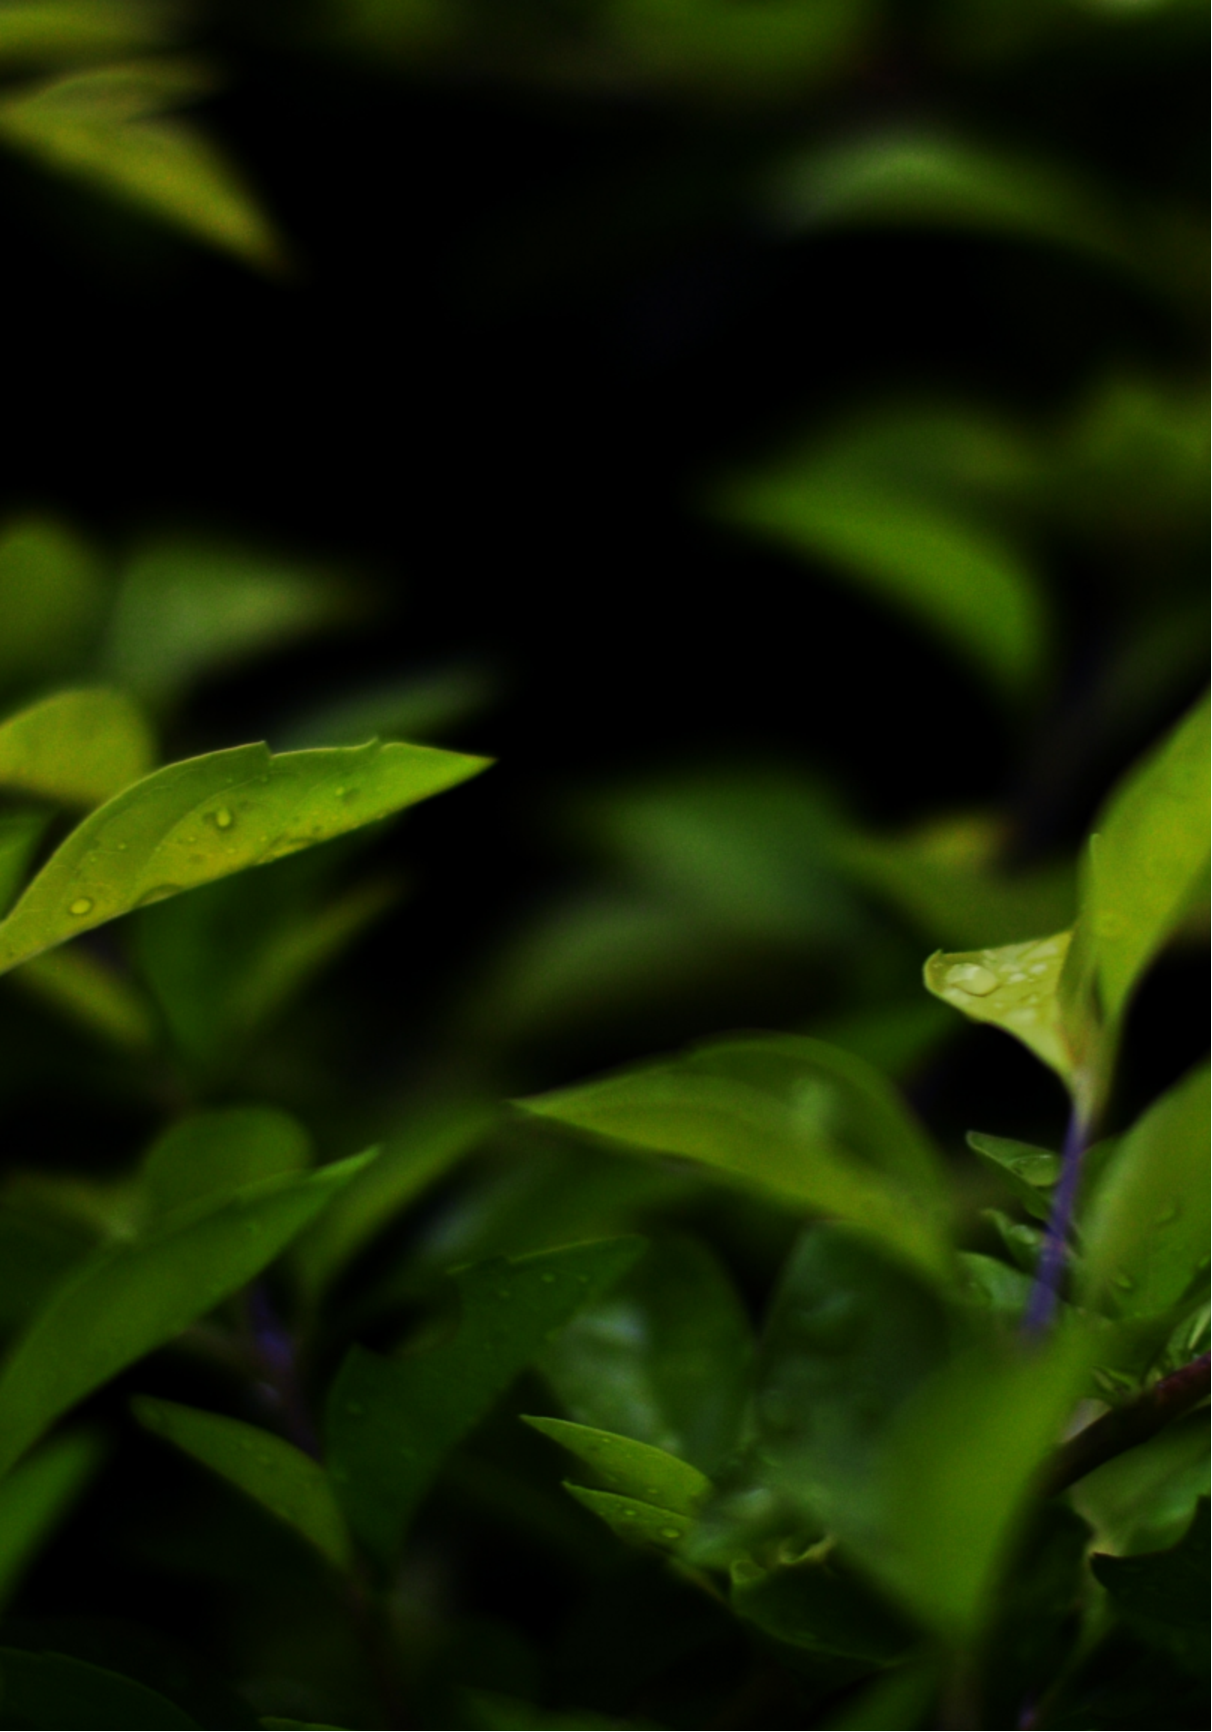
\includegraphics[width=\paperwidth]{background}}; % Background image
\draw[anchor=north] (midpoint) node 
[fill=ocre!30!white,fill opacity=0.6,text opacity=1,inner sep=1cm]
{\Huge\centering\bfseries\sffamily\parbox[c][][t]{\paperwidth}
{\centering Métodos numéricos\\[15pt] % Book title
{\Large Handbook}\\[20pt] % Subtitle
{\huge Fernando Pujaico Rivera}}}; % Author name
\end{tikzpicture}};
\end{tikzpicture}
\vfill
\endgroup

%----------------------------------------------------------------------------------------
%	COPYRIGHT PAGE
%----------------------------------------------------------------------------------------

\newpage
~\vfill
\thispagestyle{empty}

\noindent Copyright \copyright\ 2019 Fernando Pujaico Rivera\\ % Copyright notice

\noindent \textsc{Published by Virtual Books}\\ % Publisher

\noindent \textsc{book-website.com}\\ % URL

\noindent Licensed under the Creative Commons Attribution-NonCommercial 3.0 
Unported License (the ``License''). You may not use this file except in 
compliance with the License. You may obtain a copy of the License at 
\url{http://creativecommons.org/licenses/by-nc/3.0}.\\ % License information

\noindent \textit{First printing, March 2019} % Printing/edition date


%----------------------------------------------------------------------------------------
%	DEDICATORIA
%----------------------------------------------------------------------------------------

\cleardoublepage

\null
\vfill
\thispagestyle{empty}



{\normalsize \it \hfill Amicum lege feliciter, vivas, gaudeas, floreas in Deo. \vspace*{4pt}

%\hfill understanding and assistance they have given me. \vspace*{4pt}

\hfill Fernando \vspace*{4pt}}

 


%----------------------------------------------------------------------------------------
%	Acknowledgements
%----------------------------------------------------------------------------------------

\cleardoublepage

\begin{center}
\Huge{\textbf{Agradecimentos}}
\end{center}

\null
\vfill
\thispagestyle{empty}

{\normalsize \it \hfill Dou muitas graças a Deus \vspace*{4pt}}


~\\

{\normalsize \it Dou muitas graças a XXXXX XXXXXXXXX por me 
ajudar a corrigir muitos dos erros na escrita do livro.
\vspace*{4pt}}

{\normalsize \it Dou muitas graças a XXXXX XXXXXXXXX por me 
ajudar a revisar a forma da escrita na linguagem matemática do livro.
\vspace*{4pt}}

\begin{comment}
{\normalsize \it Dou muitas graças a XXXXX XXXXXXXXX por me 
ajudar a resolver muitas duvidas sobre definições e uso de termos na XXXXXXX XXXXXXX.
\vspace*{4pt}}
\end{comment}

\begin{comment}
{\normalsize \it Dou muitas graças a XXXXX XXXXXXXXX pela 
suas sugestões e revisão  do capitulo XXXXX XXXXXXXXX.
\vspace*{4pt}}
\end{comment}


 


%----------------------------------------------------------------------------------------
%	TABLE OF CONTENTS
%----------------------------------------------------------------------------------------

\chapterimage{chapter_head_1.pdf} % Table of contents heading image

\pagestyle{empty} % No headers

\tableofcontents % Print the table of contents itself

%%%%%%%%%%%%%%%%%%%%%%%%%%%%%%%%%%%%%%%%%%%%%%%%%%%%%%%%%%%%%%%%%%%%%%%%%%%%%%%%
%%%%%%%%%%%%%%%%%%%%%%%%%%%%%%%%%%%%%%%%%%%%%%%%%%%%%%%%%%%%%%%%%%%%%%%%%%%%%%%%
%%%%%%%%%%%%%%%%%%%%%%%%%%%%%%%%%%%%%%%%%%%%%%%%%%%%%%%%%%%%%%%%%%%%%%%%%%%%%%%%
%% Lista de figuras (gerada automaticamente)
\cleardoublepage
%\addcontentsline{toc}{chapter}{Lista de Figuras}
\listoffigures

%% Lista de tabelas (gerada automaticamente)
\cleardoublepage
%\addcontentsline{toc}{chapter}{Lista de Tablas}
\listoftables

%% Glossário (gerado automaticamente)
\cleardoublepage
%\renewcommand{\nomname}{Glossary}
%\addcontentsline{toc}{chapter}{\nomname}
%\markboth{GLOSSARY}{GLOSSARY}
\printnomenclature

%%% Lista de Simbolos (gerada manualmente)
\cleardoublepage
%%\addcontentsline{toc}{chapter}{LIST OF SIMBOLS}
%%\markboth{LIST OF SYMBOLS}{LIST OF SYMBOLS}
\chapter*{Lista de Símbolos}

\singlespacing

%\noindent
\section*{Tipos de Dados}
\begin{tabular}{r | p{.45\linewidth} | l}
\hline	
Tipo & Descrição & Formatação \\ \hline
$\mathbf{A}$, $\mathbf{B}$, ..., $\mathbf{X}$, $\mathbf{Y}$, $\mathbf{Z}$& Matriz. & Maiúsculo e negrito \\
$\mathbf{a}$, $\mathbf{b}$, ..., $\mathbf{x}$, $\mathbf{y}$, $\mathbf{z}$ & Vetor (Por falta é asumido que é um vetor coluna) ou conjunto. & Minúsculo e negrito \\
%$A$, $B$, ..., $X$, $Y$, $Z$ & ------- & Maiúsculo \\
$a$, $b$, ..., $x$, $y$, $z$ & Escalar variável. & Minúsculo \\
$A$, $B$, ..., $X$, $Y$, $Z$ & Escalar constante. & Minúsculo \\
$\alpha$, $\beta$, ..., $\chi$, $\psi$, $\omega$ & Escalar variável ou constante. & Letras gregas e minúsculo  \\ \hline
\end{tabular}

\section*{Elementos de matrizes bidimensionais}
\begin{tabular}{r | p{.55\linewidth} | l}
\hline	
Tipo & Descrição & Formatação \\ \hline
$a_{ij}$ & Escalar formado pelo elemento da linha $i$, coluna $j$ da matriz $\mathbf{A}$. & Minúsculo \\ \hline
%$\mathbf{A}_{(i,j)}$& Elemento na linha $i$, coluna $j$ da matriz $\mathbf{A}$ & Maiúsculo e negrito \\ \hline
%$\mathbf{a}_{i}$ & Linha ou coluna $i$-essima da matriz $\mathbf{A}$ (ambíguo) & Minúsculo e negrito \\
$a_{i:}$ & Vetor linha formado pela linha $i$-essima da matriz $\mathbf{A}$.  & Minúsculo \\
%$\mathbf{A}_{(i,:)}$& Vetor formado pela linha $i$-essima da matriz $\mathbf{A}$ & Maiúsculo e negrito \\
$a_{:i}$ & Vetor coluna formado pela coluna $i$-essima da matriz $\mathbf{A}$.  & Minúsculo \\
%$\mathbf{A}_{(:,i)}$& Vetor formado pela coluna $i$-essima da matriz $\mathbf{A}$ & Maiúsculo e negrito \\ \hline
\end{tabular}

\section*{Elementos de vetores ou conjuntos}
\begin{tabular}{r | p{.55\linewidth} | l}
\hline	
Tipo & Descrição & Formatação \\ \hline
$a_{i}$ & Elemento $i$-essimo do vetor ou conjunto  $\mathbf{a}$.& Minúsculo \\
%$\mathbf{a}_{(i)}$ & Elemento $i$-essimo do vetor $\mathbf{a}$ & Minúsculo e negrito \\ \hline
\end{tabular}

\section*{Funções notáveis}
\begin{tabular}{r | p{.70\linewidth} }
\hline	
Função & Descrição \\ \hline
$card(\mathbf{a})$ & Número de elementos, cardinalidade, do vetor ou conjunto $\mathbf{a}$. \\
$card(\mathbf{A})$ & Número de elementos, cardinalidade, da matriz $\mathbf{A}$. \\
\hline
$dim(\mathbf{a},1)$ & Primeira dimensão do vetor $\mathbf{a}$, número de linhas. \\
$dim(\mathbf{a},2)$ & Segunda dimensão do vetor $\mathbf{a}$, número de colunas. \\
$dim(\mathbf{A},1)$ & Primeira dimensão da matriz $\mathbf{A}$, número de linhas. \\
$dim(\mathbf{A},2)$ & Segunda dimensão da matriz $\mathbf{A}$, número de colunas. \\
$dim(\mathbf{A},N)$ & Dimensão $N$ da matriz $\mathbf{A}$, se não tiver retorna $0$. \\
\hline
$inv(\mathbf{A})$ & Inversa da matriz $\mathbf{A}$, é equivalente a escrever $\mathbf{A}^{-1}$. \\
$\mathbf{A}^{-1}$ & Inversa da matriz $\mathbf{A}$, é equivalente a escrever $inv(\mathbf{A})$. \\
\hline
$trans(\mathbf{a})$ & Transposta do vetor $\mathbf{a}$, é equivalente a escrever $\mathbf{a}^{T}$. \\
$\mathbf{a}^{T}$ & Transposta do vetor $\mathbf{a}$, é equivalente a escrever $trans(\mathbf{a})$. \\
$trans(\mathbf{A})$ & Transposta da matriz $\mathbf{A}$, é equivalente a escrever $\mathbf{A}^{T}$. \\
$\mathbf{A}^{T}$ & Transposta da matriz $\mathbf{A}$, é equivalente a escrever $trans(\mathbf{A})$. \\
\hline
$||\mathbf{a}||$ & Módulo do vetor $\mathbf{a}$, é equivalente a escrever $\sqrt{\sum_i a_i^2}$. \\
$||\mathbf{a}||^2$ & Módulo ao quadrado do vetor $\mathbf{a}$, 
é equivalente a escrever $\sum_i a_i^2$ ou $\mathbf{a}^{T}\mathbf{a}$ se $\mathbf{a}$ é um vetor coluna. \\
$||\mathbf{a}||_{\mathbf{B}}^2$ & Módulo ao quadrado ponderado do vetor $\mathbf{a}$, 
é equivalente a escrever $\sum_i b_{ii} a_i^2$ ou $(\sqrt{\mathbf{B}}~\mathbf{a})^{T}\sqrt{\mathbf{B}}~\mathbf{a} \equiv \mathbf{a}^{T}\mathbf{B}\mathbf{a}$ 
se $\mathbf{a}$ é um vetor coluna. Sendo que $\mathbf{B}$ é uma matriz diagonal.\\
\end{tabular}

\onehalfspacing

%%%%%%%%%%%%%%%%%%%%%%%%%%%%%%%%%%%%%%%%%%%%%%%%%%%%%%%%%%%%%%%%%%%%%%%%%%%%%%%%
%%%%%%%%%%%%%%%%%%%%%%%%%%%%%%%%%%%%%%%%%%%%%%%%%%%%%%%%%%%%%%%%%%%%%%%%%%%%%%%%
%%%%%%%%%%%%%%%%%%%%%%%%%%%%%%%%%%%%%%%%%%%%%%%%%%%%%%%%%%%%%%%%%%%%%%%%%%%%%%%%


\cleardoublepage % Forces the first chapter to start on an odd page so it's on the right

\pagestyle{fancy} % Print headers again

%----------------------------------------------------------------------------------------
%	PART
%----------------------------------------------------------------------------------------

\part{Part One}
%\chapterimage{chapter_letras.pdf} % Chapter heading image

\chapter{Notações e termos}

%%%%%%%%%%%%%%%%%%%%%%%%%%%%%%%%%%%%%%%%%%%%%%%%%%%%%%%%%%%%%%%%%%%%%%%%%%%%%%%%
%%%%%%%%%%%%%%%%%%%%%%%%%%%%%%%%%%%%%%%%%%%%%%%%%%%%%%%%%%%%%%%%%%%%%%%%%%%%%%%%
%%%%%%%%%%%%%%%%%%%%%%%%%%%%%%%%%%%%%%%%%%%%%%%%%%%%%%%%%%%%%%%%%%%%%%%%%%%%%%%%
\section{Notação usada para matrizes, vetores e funções}
\begin{notation}[Modo em que os valores escalares, vetoriais ou matriciais são definidos:]~\\
\begin{tabular}{p{.2\textwidth} | p{.4\textwidth} | p{.3\textwidth} }
\hline	
\textbf{Tipo} & \textbf{Descrição} & \textbf{Formatação} \\ \hline
$\MATRIX{A}$, $\MATRIX{B}$, ..., $\MATRIX{X}$, $\MATRIX{Y}$, $\MATRIX{Z}$& Matriz. & Maiúsculo e negrito \\
$\VECTOR{a}$, $\VECTOR{b}$, ..., $\VECTOR{x}$, $\VECTOR{y}$, $\VECTOR{z}$ & Vetor ou conjunto. & Minúsculo e negrito \\
%$A$, $B$, ..., $X$, $Y$, $Z$ & ------- & Maiúsculo \\
$a$, $b$, ..., $x$, $y$, $z$ & Escalar variável. & Minúsculo \\
$A$, $B$, ..., $X$, $Y$, $Z$ & Escalar constante. & Maiúsculo \\
$\alpha$, $\beta$, ..., $\chi$, $\psi$, $\omega$ & Escalar variável ou constante. & Letras gregas  \\ \hline
\end{tabular}
\end{notation}


\begin{notation}[Funções notáveis usadas neste livro:]~\\
\begin{tabular}{p{.11\textwidth} |  p{.8\textwidth} }
\hline	
\textbf{Função} & \textbf{Descrição} \\ \hline
%$card(\VECTOR{a})$ & Número de elementos, cardinalidade, do vetor ou conjunto $\VECTOR{a}$. \\
$card(\MATRIX{A})$ & Número de elementos, cardinalidade, da matriz $\MATRIX{A}$. \\
\hline
%$dim(\VECTOR{a},1)$ & Primeira dimensão do vetor $\VECTOR{a}$, número de linhas. \\
%$dim(\VECTOR{a},2)$ & Segunda dimensão do vetor $\VECTOR{a}$, número de colunas. \\
$dim(\MATRIX{A},1)$ & Primeira dimensão da matriz $\MATRIX{A}$, número de linhas. \\
$dim(\MATRIX{A},2)$ & Segunda dimensão da matriz $\MATRIX{A}$, número de colunas. \\
$dim(\MATRIX{A},N)$ & Dimensão $N$ da matriz $\MATRIX{A}$, se não tiver retorna $1$. \\
\hline
$\funcinv(\MATRIX{A})$ & Inversa da matriz $\MATRIX{A}$, é equivalente a escrever $\MATRIX{A}^{-1}$. \\
$\MATRIX{A}^{-1}$ & Inversa da matriz $\MATRIX{A}$, é equivalente a escrever $\funcinv(\MATRIX{A})$. \\
\hline
%$\functrans(\VECTOR{a})$ & Transposta do vetor $\VECTOR{a}$, é equivalente a escrever $\VECTOR{a}^{\transpose}$. \\
%$\VECTOR{a}^{\transpose}$ & Transposta do vetor $\VECTOR{a}$, é equivalente a escrever $trans(\VECTOR{a})$. \\
$\functrans(\MATRIX{A})$ & Transposta da matriz $\MATRIX{A}$, é equivalente a escrever $\MATRIX{A}^{\transpose}$. \\
$\MATRIX{A}^{\transpose}$ & Transposta da matriz $\MATRIX{A}$, é equivalente a escrever $trans(\MATRIX{A})$. \\
\hline
$\funcdiag(\VECTOR{a})$ & Matriz diagonal construída a partir de colocar na diagonal os elementos do vetor $\VECTOR{a}$ . \\
\hline
$\lambda_{\MATRIX{A}}$ & Matriz diagonal onde os elementos da diagonal correspondem com os autovalores da matriz $\MATRIX{A}$. \\
\hline
$det(\MATRIX{A})$ & Determinante da matriz $\MATRIX{A}$. \\
\hline
\end{tabular}
\end{notation}

\newpage
\begin{notation}[Modo em que os elementos dos vetores ou conjuntos são definidos:]
\begin{tabular}{p{.05\textwidth} | p{.6\textwidth} | p{.25\textwidth}}
\hline	
\textbf{Tipo} & \textbf{Descrição} & \textbf{Formatação} \\ \hline
$a_{i}$ & Elemento $i$-ésimo do vetor ou conjunto  $\VECTOR{a}$.& Minúsculo \\
%$\VECTOR{a}_{(i)}$ & Elemento $i$-ésimo do vetor $\VECTOR{a}$ & Minúsculo e negrito \\ \hline
\hline
\end{tabular}
\end{notation}


\begin{notation}[Modo em que os elementos das matrizes bidimensionais são definidos:]~\\
\begin{tabular}{p{.05\textwidth} | p{.6\textwidth} | p{.25\textwidth}}
\hline	
\textbf{Tipo} & \textbf{Descrição} & \textbf{Formatação} \\ \hline
$a_{ij}$ & Escalar formado pelo elemento na linha $i$, coluna $j$ da matriz $\MATRIX{A}$. & Minúsculo \\ \hline
%$\MATRIX{A}_{(i,j)}$& Elemento na linha $i$, coluna $j$ da matriz $\MATRIX{A}$ & Maiúsculo e negrito \\ \hline
%$\VECTOR{a}_{i}$ & Linha ou coluna $i$-ésima da matriz $\MATRIX{A}$ (ambíguo) & Minúsculo e negrito \\
$a_{i:}$ & Vetor linha formado pela linha $i$-ésima da matriz $\MATRIX{A}$.  & Minúsculo \\
%$\MATRIX{A}_{(i,:)}$& Vetor formado pela linha $i$-ésima da matriz $\MATRIX{A}$ & Maiúsculo e negrito \\
$a_{:i}$ & Vetor coluna formado pela coluna $i$-ésima da matriz $\MATRIX{A}$.  & Minúsculo \\
%$\MATRIX{A}_{(:,i)}$& Vetor formado pela coluna $i$-ésima da matriz $\MATRIX{A}$ & Maiúsculo e negrito \\ \hline
\hline
\end{tabular}
\end{notation}


\begin{notation}[Funções em tempo continuo e discreto:]~\\
\begin{tabular}{p{.05\textwidth} | p{.85\textwidth} }
\hline	
\textbf{Tipo}            & \textbf{Descrição} \\ \hline
$x(t)$          & Função escalar de domínio continuo, representado pela variável $t$. \\ \hline
$x[n]$          & Função escalar de domínio discreto, onde a variável $n$ representa a $n$-ésima amostra. \\ \hline
$\VECTOR{x}(t)$ & Função vetorial de domínio continuo, representado pela variável $t$.  \\ \hline
$\VECTOR{x}[n]$ & Função vetorial de domínio discreto, onde a variável $n$ representa a $n$-ésima amostra. \\
\hline
\end{tabular}
\end{notation}



%%%%%%%%%%%%%%%%%%%%%%%%%%%%%%%%%%%%%%%%%%%%%%%%%%%%%%%%%%%%%%%%%%%%%%%%%%%%%%%%
%%%%%%%%%%%%%%%%%%%%%%%%%%%%%%%%%%%%%%%%%%%%%%%%%%%%%%%%%%%%%%%%%%%%%%%%%%%%%%%%
%%%%%%%%%%%%%%%%%%%%%%%%%%%%%%%%%%%%%%%%%%%%%%%%%%%%%%%%%%%%%%%%%%%%%%%%%%%%%%%%
\section{A linguagem matemática}

\begin{description}

\item[Definição:] \index{Definição} Uma definição é uma declaração na qual as pessoas interessadas chegam a um acordo \cite[pp. 37]{solow1987como}.
Se a definição não é aceita é impossível a comunicação de temas relacionados à definição.
\begin{example}[Uso de termos em triângulos:]~\\
\begin{itemize}
\item \textbf{Definição:} Um triângulo é chamado isósceles se dois do seus lados são iguais.
\item \textbf{Definição:} Um triângulo é chamado retângulo se tem um ângulo com $90^{\circ}$.
\item \textbf{Definição:} Um angulo é chamado reto se tem  $90^{\circ}$.
\end{itemize}
\end{example}

\item[Axioma ou Postulado:] \index{Axioma} \index{Postulado} 
Uma proposição que é aceita sem uma demostração formal \cite[pp. 47]{fossa2009introducao} \cite[pp. 41]{solow1987como}.
\begin{example}[Sobre os ângulos num triângulo isósceles:]~\\
\begin{itemize}
\item \textbf{Quinto Postulado de Euclides:} Se uma reta cortar duas outras retas de modo que a soma dos dois ângulos interiores, de um mesmo lado, seja menor que dois ângulos retos, então as duas outras retas se cruzam, quando suficientemente prolongadas, do lado da primeira reta em que se acham os dois ângulos.
\end{itemize}
\end{example}

Antigamente existia uma distinção mais acentuada entre os termos axioma e postulado \cite[pp. 115]{de1863ensaio},
porém o uso popular foi acurtando a distancia entre estes dois termos \cite[pp. 243]{mora2000dicionario}.
Por exemplo, nesse antigo uso dos termos axioma e postulado, poderíamos entender estos termos como,
\begin{itemize}
\item \textbf{Axioma:} ``Isto é assim porque é evidente, não preciso demostrar''.
\item \textbf{Postulado:} ``Para futuras interações gostaria propor que partamos da base que esta afirmação é verdadeira,
 para poder chegar a conclusões decorrentes desta afirmação em nosso dialogo''.
\end{itemize}


\item[Lema:] \index{Lema} Um lema é uma proposição preliminar demostrada, 
a qual será usada para demostrar um teorema \cite[pp. 49]{fossa2009introducao}\cite[pp. 41]{solow1987como},
a afirmação indicada pelo lema não tem muita importância matemática em sim mesma, mas cumpre um papel importante para a demostração de um teorema.
Falando de forma estrita um lema também é um teorema; é dizer, uma proposição demostrada.
\begin{example}[Sobre os ângulos num triângulo isósceles:]~\\
\begin{itemize}
\item \textbf{Lema:} Num triangulo, se um angulo é reto os outros dois somam $90^{\circ}$.
\end{itemize}
\end{example}

\item[Proposição:] \index{Proposição} Uma proposição é um enunciado ou afirmação que se busca demostrar \cite[pp. 41]{solow1987como}.
\begin{example}[Sobre os ângulos num triângulo isósceles:]~\\
\begin{itemize}
\item \textbf{Proposição:} Num triangulo isósceles, uma linha que parte do vértice com lados iguais e divide ao lado oposto na metade,
forma um ângulo reto com este lado.
\end{itemize}
\end{example}

\item[Teorema:] \index{Teorema} Um teorema é uma proposição demostrada \cite[pp. 49]{fossa2009introducao} \cite[pp. 41]{solow1987como}.
\begin{example}[Sobre os ângulos num triângulo isósceles:]~\\
\begin{itemize}
\item \textbf{Teorema:} Num triangulo isósceles, uma linha que parte do vértice com lados iguais e divide ao lado oposto na metade,
forma um ângulo reto com este lado.
\item \textbf{Prova:}  Se chamamos $2\beta$ ao ângulo entre os lados iguais, 
e $\alpha$ a cada um dos ângulos restantes do triângulo isósceles. Sabendo
que a soma de ângulos num triângulo é $180^{\circ}=2\beta+2\alpha$,
concluímos que $\beta+\alpha=90^{\circ}$.
Dado que cada um dos dois triângulos formados pela divisão criada pela linha, tem ângulos $\alpha$ e $\beta$,
podemos concluir que o ângulo restante tem $90^{\circ}$, é dizer é um ângulo reto.
\end{itemize}
\end{example}

\item[Corolário:] \index{Corolário} Um corolário é uma proposição 
fácil de demostrar que se deduz a partir de um teorema \cite[pp. 49]{fossa2009introducao} \cite[pp. 41]{solow1987como}.
Falando de forma estrita um corolário também é um teorema; é dizer, uma proposição demostrada.
\begin{example}[Sobre os ângulos num triângulo isósceles:]~\\
\begin{itemize}
\item \textbf{Corolário:} Num triangulo isósceles, 
uma linha que parte do vértice com lados iguais e divide ao lado oposto na metade,
cria dois triângulos retângulos.
\end{itemize}
\end{example}

\end{description}


%%%%%%%%%%%%%%%%%%%%%%%%%%%%%%%%%%%%%%%%%%%%%%%%%%%%%%%%%%%%%%%%%%%%%%%%%%%%%%%%
%%%%%%%%%%%%%%%%%%%%%%%%%%%%%%%%%%%%%%%%%%%%%%%%%%%%%%%%%%%%%%%%%%%%%%%%%%%%%%%%
%%%%%%%%%%%%%%%%%%%%%%%%%%%%%%%%%%%%%%%%%%%%%%%%%%%%%%%%%%%%%%%%%%%%%%%%%%%%%%%%
\section{Descrição geral do problema inverso}

\index{Problema!Direto}
\index{Problema!Inverso}
Segundo o matemático Joseph B. Keller \cite{Keller76}, dois problemas são considerados inversos 
um do outro, se a formulação de cada um deles envolve a resposta do outro,
de modo que por motivos históricos, um deles é bem conhecido e estudado,
pelo que recebe o nome de \textbf{problema direto}, 
e o outro problema é novo e pouco estudado, pelo que é chamado \textbf{problema inverso}.
 
\begin{example}[Raízes e polinômios:]~
\begin{description}
\item[Problema direto -] Achar as raízes $x_{z_1}$, $x_{z_2}$, ..., $x_{z_N}$, 
conhecendo os coeficientes do polinômio $p_{\VECTOR{c}}(x)$ agrupados no vetor $\VECTOR{c}$  \cite{Keller76}.
\item[Problema inverso -] Achar os coeficientes do polinômio $p_{\VECTOR{c}}(x)$ agrupados no vetor $\VECTOR{c}$, 
conhecendo que existem raízes em $x_{z_1}$, $x_{z_2}$, ..., $x_{z_N}$ \cite{Keller76}.
\end{description}
Uma representação gráfica do problema direto pode ser vista na Figura \ref{fig:inverso-diretos:direto1}
e do problema inverso na Figura \ref{fig:inverso-diretos:inverso1};
nesses exemplos não usamos entrada de dados, 
os coeficientes do polinômio agrupados no vetor $\VECTOR{c}$ são os parâmetros do sistema e 
os valores $x_{z_n}$ pertencem aos dados de saída.
\end{example}

\begin{example}[Avaliação vs. regressão:]~
\begin{description}
\item[Problema direto -] Achar os valores $y_1$,~ $y_2$,~ ...,~ $y_N$, 
conhecendo os coeficientes do polinômio $y=p_{\VECTOR{c}}(x)$, agrupados no vetor $\VECTOR{c}$, e
os valores $x_1$, $x_2$, ..., $x_N$ \cite{Keller76}.
\item[Problema inverso -] Achar os coeficientes do polinômio $y=p_{\VECTOR{c}}(x)$ agrupados no vetor $\VECTOR{c}$, 
conhecendo que existem os valores $x_1$, $x_2$, ..., $x_N$ e 
$y_1$,~ $y_2$,~ ...,~ $y_N$  \cite{Keller76}.
\end{description}
Uma representação gráfica do problema direto pode ser visto na Figura \ref{fig:inverso-diretos:direto1}
e do problema inverso na Figura \ref{fig:inverso-diretos:inverso1}, 
em que $x_n$ pertence à entrada de dados, 
os coeficientes do polinômio agrupados no vetor $\VECTOR{c}$ são os parâmetros 
do sistema, e $y_n$ pertence aos dados de saída.
\end{example}


\begin{example}[Avaliação vs. regressão:]~
\begin{description}
\item[Problema direto -] Achar os valores $y_1$, $y_2$, ..., $y_n$, ..., $y_N$, 
que são as respostas de avaliar um valor $x$ nos polinômios 
$y=p_{\VECTOR{c}_n}(x)$ com coeficientes agrupados em vetores $\VECTOR{c}_n$ \cite{Keller76}.
\item[Problema inverso -] Achar o valor $x$
conhecendo vários polinômios $y=p_{\VECTOR{c}_n}(x)$ com coeficientes agrupados em vetores $\VECTOR{c}_n$ e
os resultados $y_1$, $y_2$, ..., $y_n$, ..., $y_N$  \cite{Keller76}.
\end{description}
Uma representação gráfica do problema direto pode ser vista na Figura \ref{fig:inverso-diretos:direto1}
e do problema inverso na Figura \ref{fig:inverso-diretos:inverso2}.
\end{example}

\begin{figure}[!h]
     \centering
     \begin{subfigure}[b]{0.49\textwidth}
         \centering
         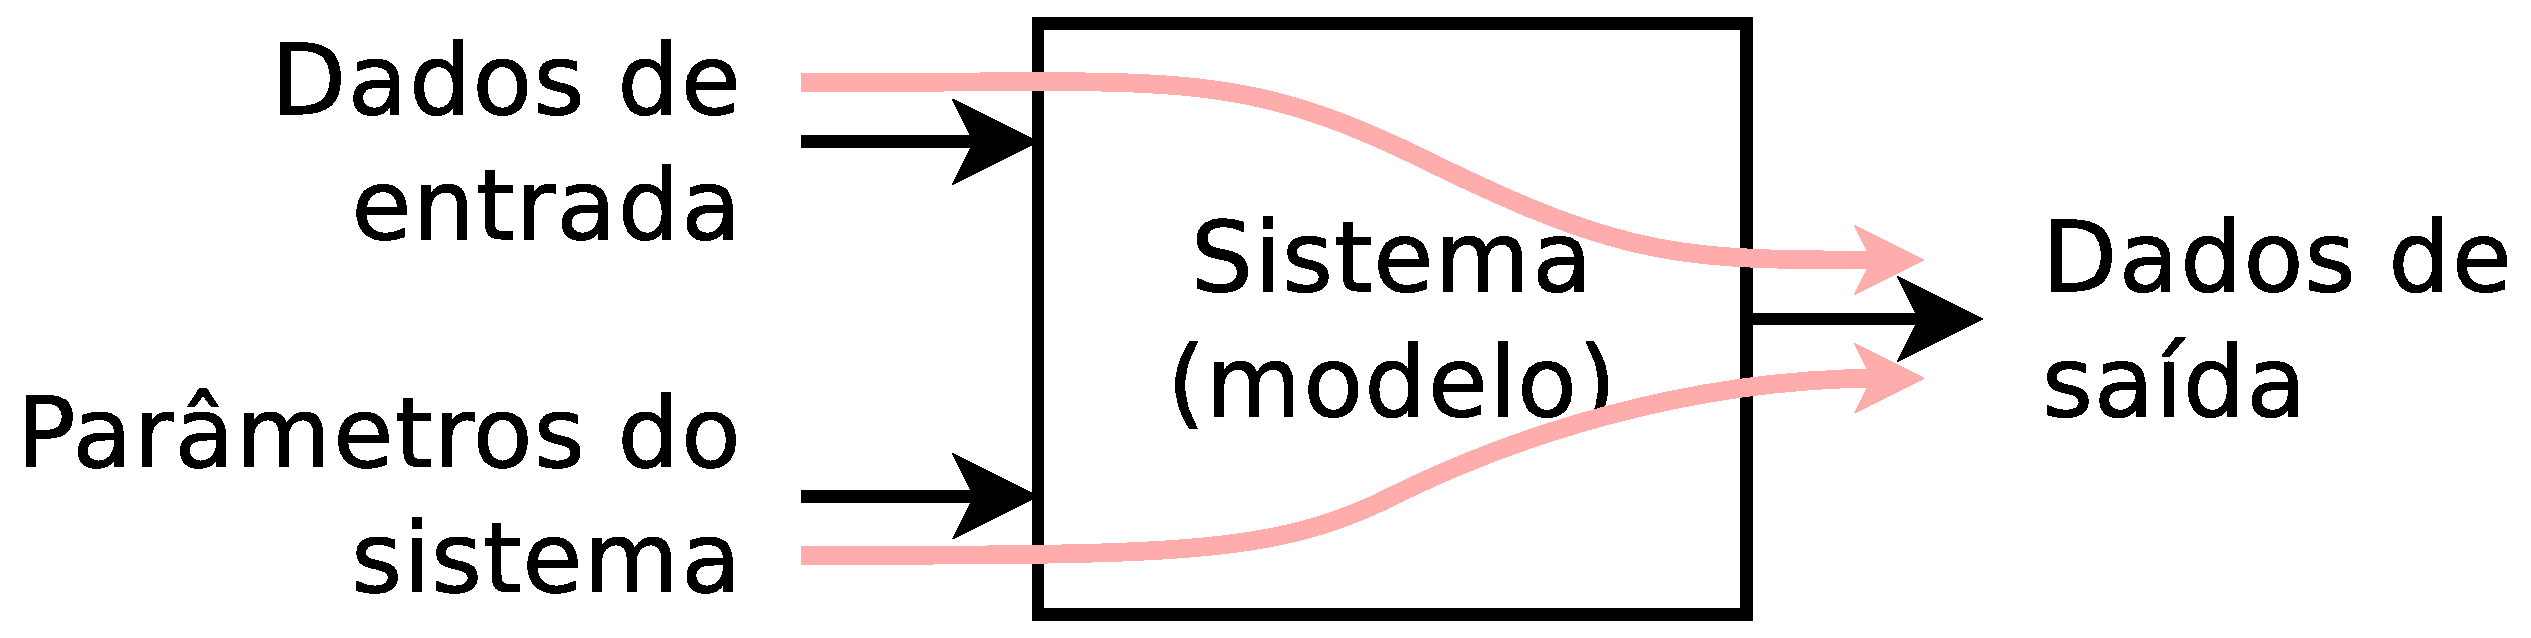
\includegraphics[width=0.95\textwidth]{chapters/notacao/direto1.eps}
         \caption{Problema direto.}
         \label{fig:inverso-diretos:direto1}
     \end{subfigure}
     \hfill
     \begin{subfigure}[b]{0.49\textwidth}
         \centering
         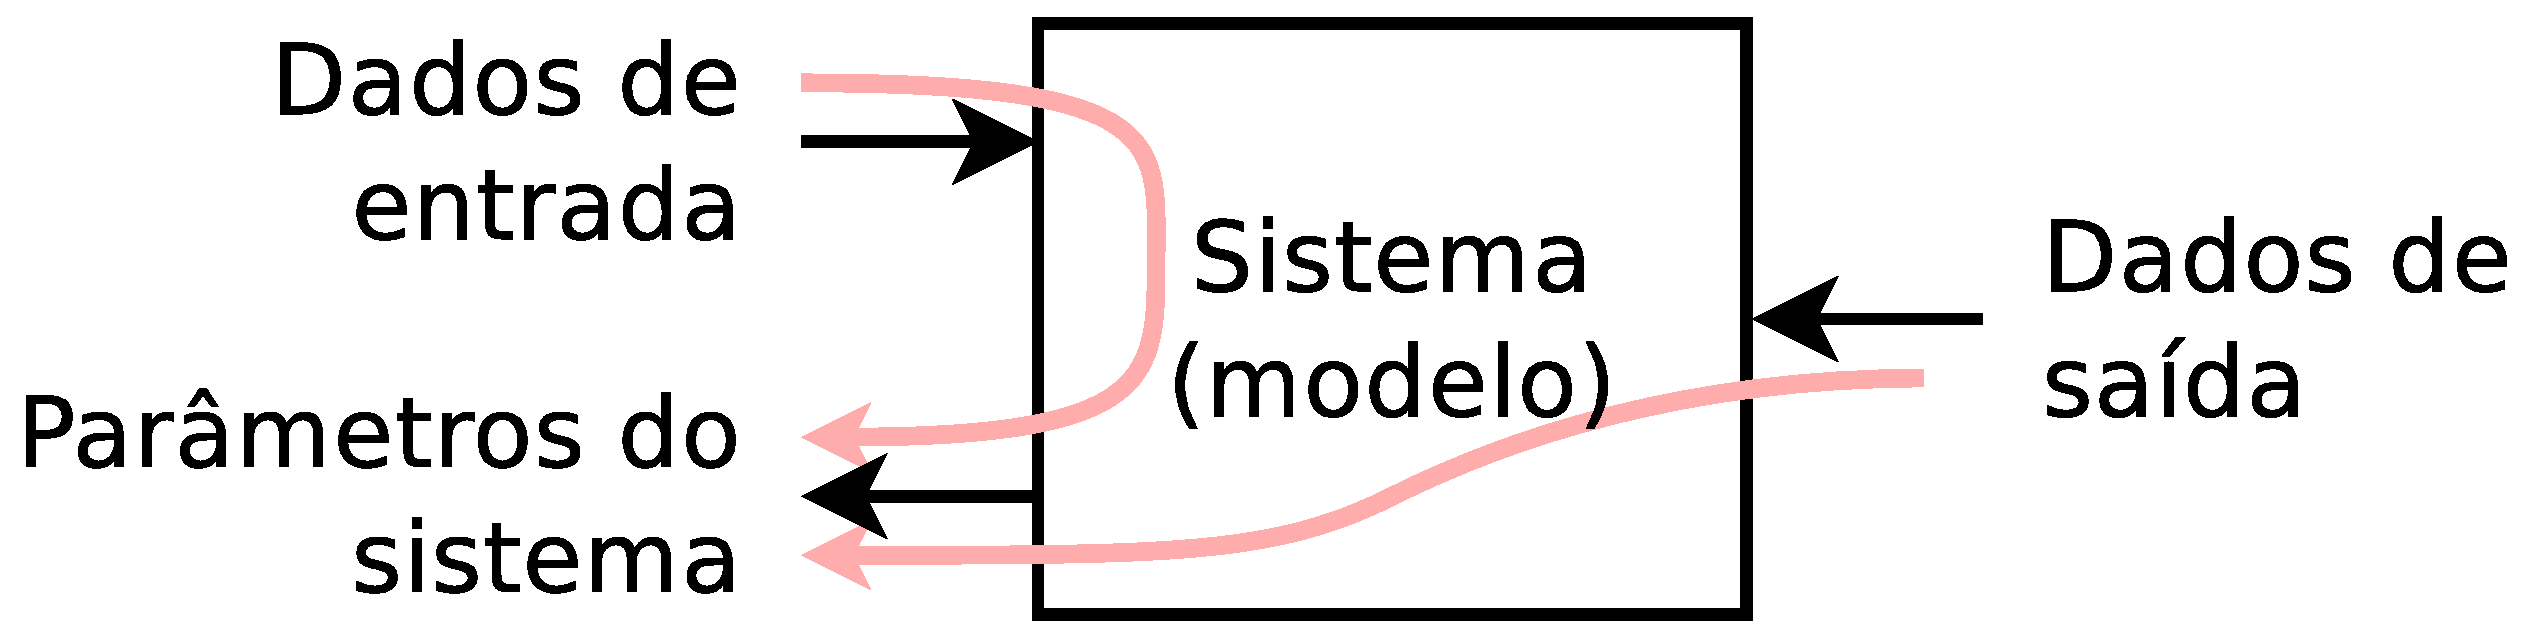
\includegraphics[width=0.95\textwidth]{chapters/notacao/inverso1.eps}
         \caption{Problema inverso.}
         \label{fig:inverso-diretos:inverso1}
     \end{subfigure}
     \hfill
     \begin{subfigure}[b]{0.49\textwidth}
         \centering
         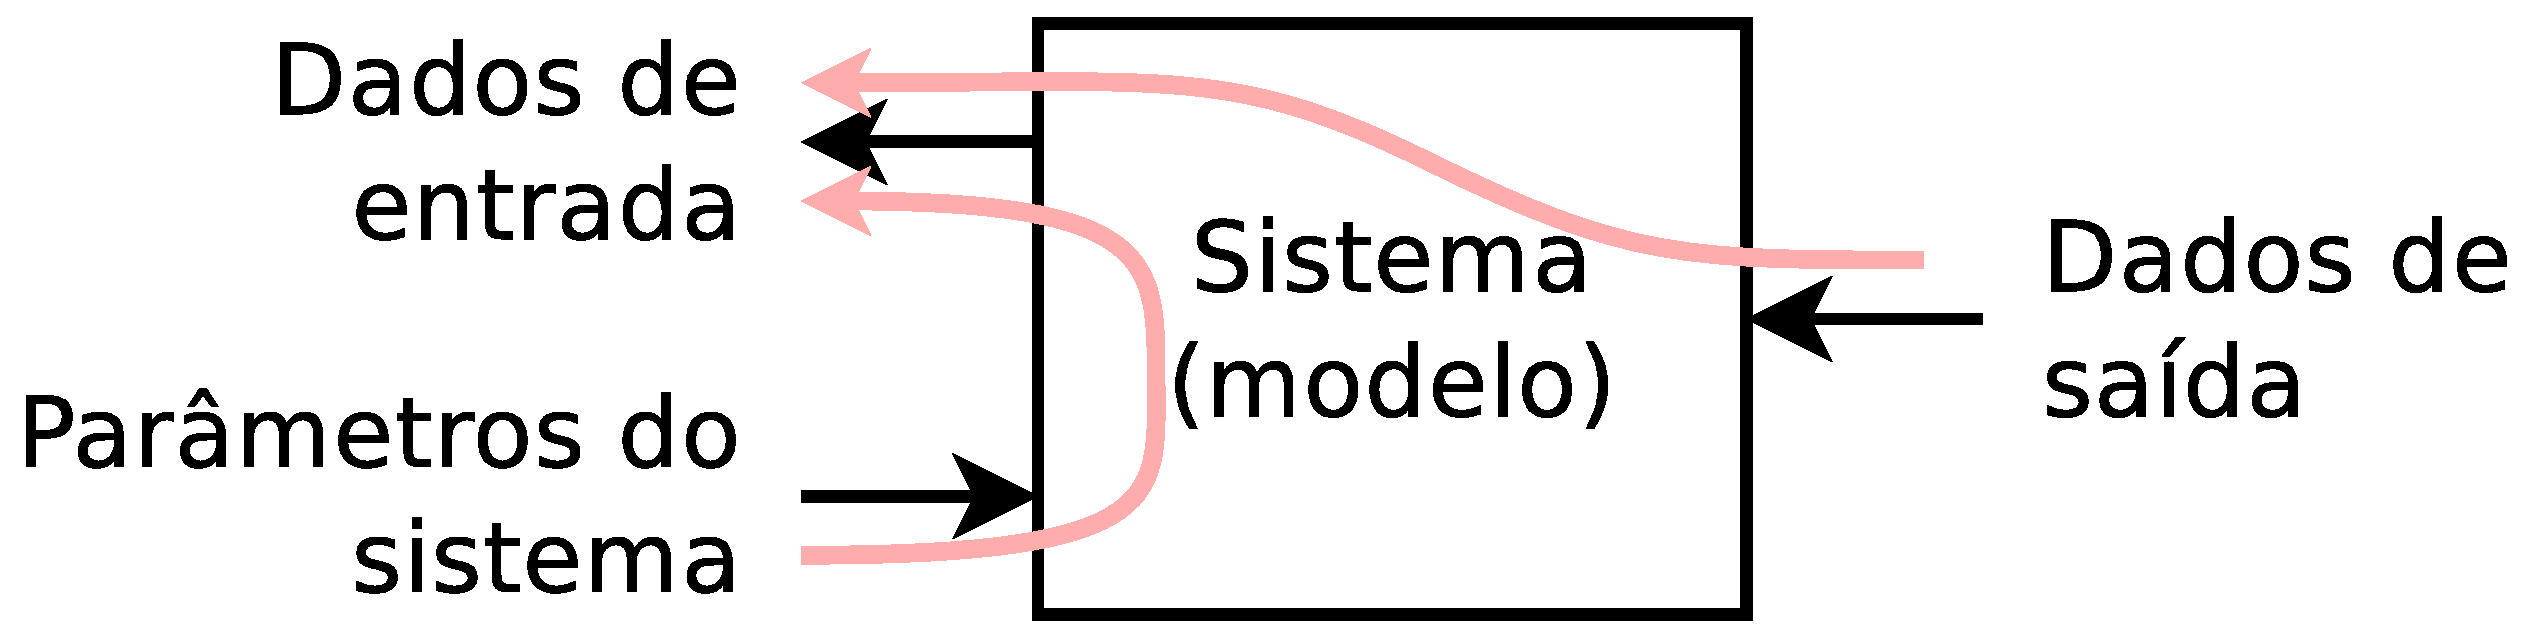
\includegraphics[width=0.95\textwidth]{chapters/notacao/inverso2.eps}
         \caption{Problema inverso.}
         \label{fig:inverso-diretos:inverso2}
     \end{subfigure}
        \caption{Exemplos de problemas diretos e inversos.}
        \label{fig:inverso-diretos}
\end{figure}


%%%%%%%%%%%%%%%%%%%%%%%%%%%%%%%%%%%%%%%%%%%%%%%%%%%%%%%%%%%%%%%%%%%%%%%%%%%%%%%%
%%%%%%%%%%%%%%%%%%%%%%%%%%%%%%%%%%%%%%%%%%%%%%%%%%%%%%%%%%%%%%%%%%%%%%%%%%%%%%%%
%%%%%%%%%%%%%%%%%%%%%%%%%%%%%%%%%%%%%%%%%%%%%%%%%%%%%%%%%%%%%%%%%%%%%%%%%%%%%%%%
\section{Problema \wellposed~ vs. \illposed }

%%%%%%%%%%%%%%%%%%%%%%%%%%%%%%%%%%%%%%%%%%%%%%%%%%%%%%%%%%%%%%%%%%%%%%%%%%%%%%%%
\subsection{Problema \wellposed}
\index{Problema!\Wellposed}
\index{Well-posed}
\begin{definition}[Problema \wellposed:]
\label{def:bem-posto:1}
Conhecido um modelo matemático ou sistema que desejamos manipular para obter uma solução;
indicamos que este é um problema \wellposed~ (do inglês ``well-posed'') 
quando se cumprem 3 condições\footnote{A primeira definição de um problema \wellposed~ foi realizada pelo matemático J. S. Hadamard, 
para mais detalhes sobre Hadamard ver a Pag. \pageref{elab:Hadamard}.} \cite[pp. 16]{gockenbach2016linear}
\cite[pp. 6]{p2011well}.
\begin{itemize}
\item \textbf{Existência:} Existe uma solução que verifica o sistema.
\item \textbf{Unicidade:} A solução é única.
\item \textbf{Estabilidade:} A solução depende continuamente da saída;
é dizer, pequenas variações na resposta provem de pequenas variações nos dados usados para calcular a resposta.
\end{itemize}
\end{definition}

\begin{example}[Problema \wellposed:]
Conhecido o problema de obter o vetor $\VECTOR{x} \in \mathbb{R}^{N}$,
que cumpre o sistema, $\MATRIX{A}\VECTOR{x}=\VECTOR{y}$,
 tendo como dados o vetor $\VECTOR{y} \in \mathbb{R}^{N}$ e 
a matriz $\MATRIX{A}: \mathbb{R}^{N} \rightarrow \mathbb{R}^{N}$ que carateriza ao sistema.
Falamos que o problema está \wellposed~ se a matriz $\MATRIX{A}$ tem inversa e esta é limitada \cite[pp. 18]{gockenbach2016linear}. 
\end{example}

%%%%%%%%%%%%%%%%%%%%%%%%%%%%%%%%%%%%%%%%%%%%%%%%%%%%%%%%%%%%%%%%%%%%%%%%%%%%%%%%
\subsection{Problema \illposed}
\index{Ill-posed}
\index{Problema!\Illposed}
\begin{definition}[Problema \illposed:]
\label{def:mal-posto:1}
Um problema é chamado \illposed~ (do inglês ``ill-posed'') se não cumpre um o mais das condições que definem a um problema 
\wellposed~ \cite[pp. 18]{gockenbach2016linear}.
Os problemas inversos geralmente são relacionados a um problema \illposed,
pois pelo geral não cumprem uma ou mais das condições para ser catalogados como \wellposed. 
\end{definition}

\begin{example}[Problema \illposed~ sem solução:]
\label{ex:IllPosedNoSolutions}
Conhecido o problema de obter o vetor $\VECTOR{x}\in \mathbb{R}^N$,
que cumpre o sistema,
\begin{equation}
\MATRIX{A}\VECTOR{x}=\VECTOR{y},
\qquad
\MATRIX{A}=
\begin{bmatrix}
1 & 1\\
2 & 1\\
0 & 1
\end{bmatrix}
\qquad
\VECTOR{y}=
\begin{bmatrix}
2\\
3\\
2
\end{bmatrix};
\end{equation}
catalogamos este problema como \illposed~ pois não existe um vetor $\VECTOR{x}$
que verifique o sistema $\MATRIX{A}\VECTOR{x}=\VECTOR{y}$.
\end{example}


\begin{example}[Problema \illposed~com múltiplas soluções:]
\label{ex:IllPosedMultiplaSolutions}
Conhecido o problema de obter o vetor $\VECTOR{x}\in \mathbb{R}^N$,
que cumpre o sistema,
\begin{equation}
\MATRIX{A}\VECTOR{x}=\VECTOR{y},
\qquad
\MATRIX{A}=
\begin{bmatrix}
1 & 1\\
1 & 1\\
1 & 1
\end{bmatrix}
\qquad
\VECTOR{y}=
\begin{bmatrix}
2\\
2\\
2
\end{bmatrix};
\end{equation}
catalogamos este problema como \illposed~  pois existem múltiplas soluções $\VECTOR{x}$
que cumprem o sistema,
$
\VECTOR{x}=
\begin{bmatrix}
2 & 0
\end{bmatrix}^{\transpose}
+\alpha
\begin{bmatrix}
-1 & 1
\end{bmatrix} ^{\transpose}$,
$ \forall \alpha \in \mathbb{R}$.
\end{example}

\index{Hadamard, Jacques Salomon}
\begin{elaboracion}[title=Jacques Salomon Hadamard (1865-1963), width= 0.99\linewidth]
\label{elab:Hadamard}
\noindent
\begin{minipage}{0.2\linewidth}
\centering
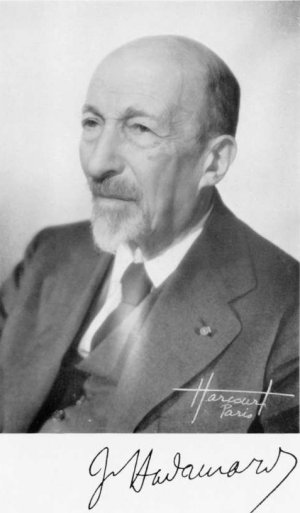
\includegraphics[width=0.98\textwidth]{chapters/notacao/Hadamard2.jpg}
\end{minipage}
\begin{minipage}{0.8\linewidth}
Notável matemático francês  e um membro da Royal Society;
durante seus primeiros anos de vida, 
Jacques se destacou em todas as disciplinas, exceto em matemática;
sua habilidade nesta área melhorou notavelmente após sua admissão no Lycée Louis-le-Grand em 1876;
logo de vários anos, cheios de  grandes realizações acadêmicas, ele completou seu Ph.D. em 1892 
e recebeu o prêmio Grand Prix de Ciências Matemáticas por seu ensaio inovador sobre a função zeta de Riemann
\cite[pp. 326]{agarwal2014creators}.
Entre suas muitas contribuições à matemática está a definição inicial de um problema \wellposed,
e consequentemente a de um problema \illposed~\cite[pp. 9, 132]{p2011well}.
\end{minipage}
\end{elaboracion}

\begin{comment}
\begin{tcbinformation} 
\textbf{Hadamard e os problemas \illposed:} 
O matemático Jacques Salomon Hadamard fez a definição inicial de um problema \wellposed,
e consequentemente a de um problema \illposed; 
ele  indicou como irrelevantes para a física ou para as aplicações do mundo real
a qualquer problema catalogado como \illposed; porém,
quatro décadas após sua declaração esta afirmação ele provou estar errado  \cite[pp. 4]{siddiqi2011mathematics}.
\end{tcbinformation} 
\end{comment}



%%%%%%%%%%%%%%%%%%%%%%%%%%%%%%%%%%%%%%%%%%%%%%%%%%%%%%%%%%%%%%%%%%%%%%%%%%%%%%%%
%%%%%%%%%%%%%%%%%%%%%%%%%%%%%%%%%%%%%%%%%%%%%%%%%%%%%%%%%%%%%%%%%%%%%%%%%%%%%%%%
%%%%%%%%%%%%%%%%%%%%%%%%%%%%%%%%%%%%%%%%%%%%%%%%%%%%%%%%%%%%%%%%%%%%%%%%%%%%%%%%
\section{Regularização}




A regularização é o processo pelo qual um problema \illposed~
é aproximado por uma família vizinha de problemas \wellposed~
\cite[pp. 49]{engl2000regularization},
para realizar esta aproximação, informação adicional é considerada no problema.


Assim, por exemplo, podemos aplicar a regularização agregando uma função objetivo para obter um problema de otimização.

\textbf{Problema direto:} Considere um sistema representado pelo seguinte problema direto,
\begin{equation}\label{eq:regularization:1}
\MATRIX{A}\VECTOR{x}=\VECTOR{y},
\end{equation}
onde a resposta vector $\VECTOR{y}\in \mathbb{R}^M$ é obtida logo de introduzir o estimulo $\VECTOR{x}\in \mathbb{R}^N$,
sendo $\MATRIX{A}:\mathbb{R}^N \rightarrow \mathbb{R}^M$ uma matriz operador lineal.

\textbf{Problema inverso:} Assim, o problema inverso para o sistema da Eq. (\ref{eq:regularization:1}), é
achar o vetor de entrada $\VECTOR{x}$, que cumpra  a Eq. (\ref{eq:regularization:2})
onde $\VECTOR{y}_{\delta}$ é um vetor com amostras ruidosas de $\VECTOR{y}$,
e $0\leq||\VECTOR{y}-\VECTOR{y}_{\delta}||^2\leq \delta^2$.
\begin{equation}\label{eq:regularization:2}
\MATRIX{A}\VECTOR{x}=\VECTOR{y}_{\delta}
\end{equation}
\begin{itemize}
\item Se o sistema da Eq. (\ref{eq:regularization:2}) estiver \wellposed,
então a solução é $\VECTOR{x}=\MATRIX{A}^{-1}\VECTOR{y}_{\delta}$ sem $M=N$,
ou $\VECTOR{x}=\left\{\MATRIX{A}^{\transpose}\MATRIX{A}\right\}^{-1}\MATRIX{A}^{\transpose}\VECTOR{y}_{\delta}$ se $M\neq N$.
\item Porem, se o problema da Eq. (\ref{eq:regularization:2}) estiver \illposed,
então não é possível obter solução.
\end{itemize}~\\
Dado que num problema  \illposed~ não podemos achar uma solução, nova informação é agregada ao problema,
pelo que no caso da Eq. (\ref{eq:regularization:2}) 
a regularização consiste em aceitar a impossibilidade da igualdade, 
e transformar esta numa função de custo usando o critério do mínimo erro quadrático,
onde definimos  $e(\VECTOR{x})$,
\begin{equation}\label{eq:regularization:3}
e(\VECTOR{x})=||\MATRIX{A}\VECTOR{x}-\VECTOR{y}_{\delta}||^2,
\end{equation}
de modo que agregamos a restrição de que a solução vetor $\VECTOR{x}$ que procuramos,
deve minimizar a função de custo $e(\VECTOR{x})$.
Na Seção \ref{sec:minAxbCAxb} veremos mais a detalhe como resolver o problema da minimização.

%%%%%%%%%%%%%%%%%%%%%%%%%%%%%%%%%%%%%%%%%%%%%%%%%%%%%%%%%%%%%%%%%%%%%%%%%%%%%%%%
%%%%%%%%%%%%%%%%%%%%%%%%%%%%%%%%%%%%%%%%%%%%%%%%%%%%%%%%%%%%%%%%%%%%%%%%%%%%%%%%
%%%%%%%%%%%%%%%%%%%%%%%%%%%%%%%%%%%%%%%%%%%%%%%%%%%%%%%%%%%%%%%%%%%%%%%%%%%%%%%%
\section{Regressão}

\index{Regressão}

\begin{wrapfigure}{l}{0.5\textwidth}
     \centering
     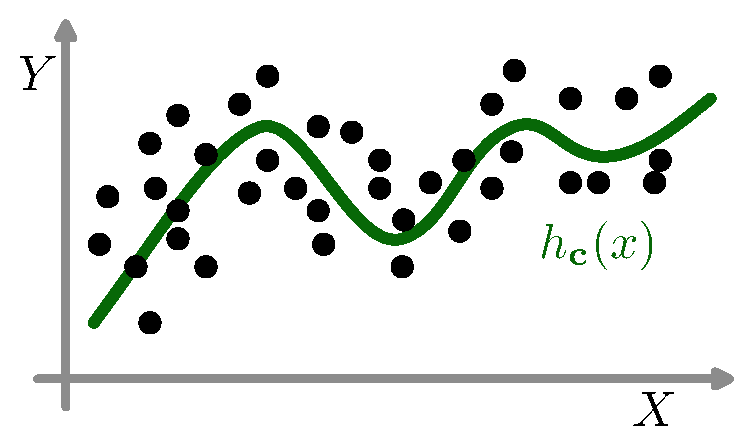
\includegraphics[width=0.45\textwidth]{chapters/notacao/regressao1.eps}
     \caption{Regressão de uma curva $h_{\VECTOR{c}}(x)$ com parâmetros $\VECTOR{c}$ num conjunto de dados. }
     \label{fig:regressao:1}
    \hspace{20pt}
\end{wrapfigure}
A regressão é o processo pelo qual uma curva ou superfície em múltiplas dimensões é 
ajustada num conjunto de dados, quando se sabe ou se aceita que existirá um erro no ajuste
devido à natureza ruidosa dos dados \cite[pp. 5]{chapra2016metodos}.

A ideia geral da regressão é achar uma curva de ajuste que represente melhor 
os dados, sem que a curva necessariamente coincida de forma exata com todos eles,
pelo que devemos definir algum critério de medida do erro de ajuste 
e procurar uma curva que minimize esse erro \cite[pp. 7]{chapra2016metodos}.

Assim, a regressão pode ser classificada mediante o tipo de curva de ajuste que é usado;
nesse sentido, podemos verificar na literatura:

\begin{itemize}
\item \textbf{Regressão linear}: 
Este caso ocorre quando usamos uma linha reta;
sendo esta uma função $h_{\VECTOR{c}}:\mathbb{R} \rightarrow \mathbb{R}$ de parâmetros $\VECTOR{c}$, 
utilizada para aproximar um conjunto de dados \cite[pp. 398, 402]{chapra2016metodos} \cite[pp. 25]{aster2013parameter}.
A regressão linear é um caso particular da regressão polinomial quando $M=1$.
\begin{example}~
\begin{itemize}
\item Curva de ajuste na regressão linear, 
\begin{equation}
h_{\VECTOR{c}}(x)=c_1+c_2 x.
\end{equation}
\item Na Seção \ref{sec:theo:reglogr1r1:1}, após uma linearização de uma relação não linear,
como na função logística, podemos ver exemplos de regressão linear.
\end{itemize}
\end{example}

\item \textbf{Regressão polinomial}: 
Indica que usamos um polinômio de grau $M$,
sendo esta uma função $h_{\VECTOR{c}}:\mathbb{R} \rightarrow \mathbb{R}$ com parâmetros $\VECTOR{c}$, 
utilizada para aproximar um conjunto de dados \cite[pp. 399, 415]{chapra2016metodos}.
\begin{example}~
\begin{itemize}
\item Curva de ajuste na regressão polinomial com grau $M=2$,
\begin{equation}
h_{\VECTOR{c}}(x)=c_1+c_2 x+c_3 x^2.
\end{equation}
\item Na Seção \ref{sec:theo:maphxr1r1}, podemos ver exemplos de regressão polinomial.
\item Na Seção \ref{sec:theo:reglogr1r1poly:1} após uma linearização de uma relação não linear,
como na função logística, podemos ver exemplos de regressão polinomial.
\end{itemize}
\end{example}

\item \textbf{Regressão não linear}: 
Neste caso, usamos um ajuste de dados
com uma função $h_{\VECTOR{c}}:\mathbb{R} \rightarrow \mathbb{R}$ com parâmetros $\VECTOR{c}$, 
que representa uma relação não linear entre o domínio e o contradomínio de $h_{\VECTOR{c}}$ 
\cite[pp. 424]{chapra2016metodos} \cite[pp. 217]{agarwal2014creators}.
\begin{example}~
\begin{itemize}
\item Um caso de curva de ajuste na regressão não linear, 
\begin{equation}
h_{\VECTOR{c}}(x)=c_1 e^{-c_2 x}.
\end{equation}
\item Na Seção \ref{sec:theo:maphcxr1r1}, podemos ver exemplos de regressão não linear.
\end{itemize}
\end{example}

\item \textbf{Regressão linear múltipla}:
Temos este caso quando ajustamos um hiperplano;
sendo esta uma função $h_{\VECTOR{c}}:\mathbb{R}^{N} \rightarrow \mathbb{R}$ com parâmetros $\VECTOR{c}$, 
utilizada para aproximar um conjunto de dados \cite[pp. 399, 418]{chapra2016metodos}.
A regressão linear é um caso particular da regressão linear múltipla quando $N=1$.
\begin{example}~
\begin{itemize}
\item Curva de ajuste na regressão linear múltipla com $N=2$, 
\begin{equation}
h_{\VECTOR{c}}(\VECTOR{x})=c_1+c_2 x_1+c_3 x_2.
\end{equation}
\item Na Seção \ref{sec:theo:reglogrnr1:1}, após uma linearização de uma relação não linear,
como na função logística, podemos ver exemplos de regressão linear múltipla.
\end{itemize}
\end{example}

\item \textbf{Regressão polinomial múltipla}:
Acontece quando ajustamos um polinômio multivariado de grau total $M$,
sendo esta uma função $h_{\VECTOR{c}}:\mathbb{R}^{N} \rightarrow \mathbb{R}$ com parâmetros $\VECTOR{c}$, 
utilizada para aproximar um conjunto de dados.
A regressão polinomial é um caso particular da regressão polinomial múltipla quando $N=1$.
\begin{example}~
\begin{itemize}
\item Um caso de curva de ajuste na regressão polinomial múltipla com 
$N=2$ e $h_{\VECTOR{c}}:\mathbb{R}^{2} \rightarrow \mathbb{R}$, 
\begin{equation}
h_{\VECTOR{c}}(\VECTOR{x})=c_1+c_2 x_1+c_3 x_2+c_4 x_1^2+c_5 x_2^2+c_6 x_1 x_2.
\end{equation}
\item Nas Seções \ref{sec:theo:maphxr2r1} e \ref{sec:theo:maphxr2r2},
 podemos ver exemplos de regressão polinomial múltipla.
\item Na Seção \ref{sec:theo:reglogrnr1poly:1}, após uma linearização de uma relação não linear,
como na função logística, podemos ver exemplos de regressão polinomial múltipla.
\end{itemize}
\end{example}

\item \textbf{Regressão não linear múltipla}: 
Estamos neste caso quado usamos no ajuste dos dados
uma função $h_{\VECTOR{c}}:\mathbb{R}^{N} \rightarrow \mathbb{R}$, 
que representa uma função não linear entre o domínio e o contradomínio de $h_{\VECTOR{c}}$.
A regressão não linear é um caso particular da regressão não linear múltipla quando $N=1$.
\begin{example}~
\begin{itemize}
\item Um caso de curva de ajuste na regressão não linear múltipla, 
\begin{equation}
h_{\VECTOR{c}}(\VECTOR{x})=c_1 e^{- c_2^2(x_1 -c_3)^2- c_4^2(x_2 -c_5)^2}.
\end{equation}
\item Na Seção \ref{sec:theo:maphcxrnr1}, podemos ver exemplos de regressão não linear múltipla.
\item Na Seção \ref{sec:theo:reglogrnr1nolinear:1}, após uma linearização de uma relação não linear,
como na função logística, podemos ver exemplos de regressão não linear múltipla.
\end{itemize}
\end{example}
\end{itemize}

\subsection{Linearização de curvas de ajuste não lineares}

Os problemas de \textbf{regressão não linear}
em alguns casos podem ser modificados para ter a forma de um 
problema de \textbf{regressão linear} (simples ou múltipla);
essa caraterística é interessante, pois geralmente
os problemas não lineares são resolvidos com métodos iterativos,
que podem ou não convergir na solução.
Em contrapartida, em problemas de regressão linear,
os métodos disponíveis nos brindam com uma resposta mediante um procedimento 
predeterminado, 
o que facilita o planejamento de um procedimento de solução e favorece o tempo de computo.

Assim, na continuação mostramos 
como problemas não lineares podem ser 
adaptados a um problema de regressão linear (simples):
\begin{example}
Usando 
$\hat{y}=ln(y)$,  
$\hat{x}=ln(x)$, 
$\hat{c}_1=ln(c_1)$, e
$\hat{c}_2=c_2$, obtemos %$\hat{y}=\hat{c}_1+\hat{c}_2 \hat{x}$.
\begin{equation}
y=c_1x^{c_2}
\quad \rightarrow \quad 
\hat{y}=\hat{c}_1+\hat{c}_2 \hat{x}.
\end{equation}
\vspace{-2pt}
\end{example}

\begin{example}%[Curva de ajuste $y=c_1 {c_2}^x$:]
Usando 
$\hat{y}=ln(y)$,  
$\hat{x}=x$, 
$\hat{c}_1=ln(c_1)$, e
$\hat{c}_2=ln(c_2)$, obtemos %$\hat{y}=\hat{c}_1+\hat{c}_2 \hat{x}$.
\begin{equation}
y=c_1 {c_2}^x
\quad \rightarrow \quad 
\hat{y}=\hat{c}_1+\hat{c}_2 \hat{x}.
\end{equation}
\vspace{-2pt}
\end{example}

\begin{example}%[Curva de ajuste $y=\left(c_1 + {c_2} x \right)^{-1}$:]
Usando 
$\hat{y}=\frac{1}{y}$,  
$\hat{x}=x$, 
$\hat{c}_1=c_1$, e 
$\hat{c}_2=c_2$, obtemos %$\hat{y}=\hat{c}_1+\hat{c}_2 \hat{x}$.
\begin{equation}
y=\left(c_1 + {c_2} x \right)^{-1}
\quad \rightarrow \quad 
\hat{y}=\hat{c}_1+\hat{c}_2 \hat{x}.
\end{equation}
\vspace{-2pt}
\end{example}

\begin{example}%[Curva de ajuste $y=c_1 x \left(c_2 + x\right)^{-1}$:] 
Usando 
$\hat{y}=\frac{1}{y}$,  
$\hat{x}=\frac{1}{x}$, 
$\hat{c}_1=\frac{1}{c_1}$, e 
$\hat{c}_2=\frac{c_2}{c_1}$, obtemos %$\hat{y}=\hat{c}_1+\hat{c}_2 \hat{x}$.
\begin{equation}
y=c_1 x \left(c_2 + x\right)^{-1}
\quad \rightarrow \quad 
\hat{y}=\hat{c}_1+\hat{c}_2 \hat{x}.
\end{equation}
\vspace{-2pt}
\end{example}

De forma similar ao caso de regressão linear simples,
curvas de ajuste não lineares podem ser adaptadas a um problema de regressão linear múltipla:
\begin{example}%[Curva de ajuste $y=c_1 +c_2 x + c_3 x^2 + c_4 x^3$:]
Usando 
$\hat{y}=y$,  
$\hat{x}_1=x$,
$\hat{x}_2=x^2$,
$\hat{x}_3=x^3$, 
$\hat{c}_1=c_1$, 
$\hat{c}_2=c_2$, 
$\hat{c}_3=c_3$, e 
$\hat{c}_4=c_4$, obtemos %$\hat{y}=\hat{c}_1+\hat{c}_2 \hat{x}_1+\hat{c}_2 \hat{x}_2+\hat{c}_3 \hat{x}_3$.
\begin{equation}
y=c_1 +c_2 x + c_3 x^2 + c_4 x^3
\quad \rightarrow \quad 
\hat{y}=\hat{c}_1+\hat{c}_2 \hat{x}_1+\hat{c}_2 \hat{x}_2+\hat{c}_3 \hat{x}_3.
\end{equation}
\vspace{-2pt}
\end{example}

\begin{example}%[Curva de ajuste $y=c_1 +c_2 \sqrt{x} + c_3 sin(x)$:]
Usando 
$\hat{y}=y$,  
$\hat{x}_1=\sqrt{x}$,
$\hat{x}_2=sin(x)$, 
$\hat{c}_1=c_1$, 
$\hat{c}_2=c_2$, e 
$\hat{c}_3=c_3$, obtemos %$\hat{y}=\hat{c}_1+\hat{c}_2 \hat{x}_1+\hat{c}_2 \hat{x}_2$.
\begin{equation}
y=c_1 +c_2 \sqrt{x} + c_3 sin(x)
\quad \rightarrow \quad 
\hat{y}=\hat{c}_1+\hat{c}_2 \hat{x}_1+\hat{c}_2 \hat{x}_2.
\end{equation}
\vspace{-2pt}
\end{example}


\newpage
%%%%%%%%%%%%%%%%%%%%%%%%%%%%%%%%%%%%%%%%%%%%%%%%%%%%%%%%%%%%%%%%%%%%%%%%%%%%%%%%
%%%%%%%%%%%%%%%%%%%%%%%%%%%%%%%%%%%%%%%%%%%%%%%%%%%%%%%%%%%%%%%%%%%%%%%%%%%%%%%%
%%%%%%%%%%%%%%%%%%%%%%%%%%%%%%%%%%%%%%%%%%%%%%%%%%%%%%%%%%%%%%%%%%%%%%%%%%%%%%%%
\section{Norma e produto interno}

A norma e o produto interno hermitiano são descritos de forma geral
na Definição \ref{def:normageral} e \ref{def:innergeral}, respetivamente.

\index{Norma em $V$!$\NORM{\VECTOR{x}}$}
\begin{definition}[Norma 
$\|\VECTOR{x}\|$ de um vetor $\VECTOR{x}$:]
\label{def:normageral}
Dado um espaço vetorial real ou complexo $V$,
a norma $\|\VECTOR{x}\|$ de um vetor $\VECTOR{x} \in V$ 
é uma função $V \rightarrow  \mathbb{R}$ 
que cumpre as seguintes três propriedades 
para todo $\VECTOR{x},\VECTOR{x}_1,\VECTOR{x}_2 \in V$ e $\alpha \in \mathbb{C}$ 
\cite[pp. 43]{d2019hermitian} \cite[pp. 27]{vetterli2014foundations}:
\begin{itemize}
\item $\|\VECTOR{x}\|> 0$ para todo vetor $\VECTOR{x}$ não nulo.
\item $\|\alpha \VECTOR{x}\|= |\alpha|~\|\VECTOR{x}\|$.
\item (Desigualdade triangular)  $\|\VECTOR{x}_1 + \VECTOR{x}_2\|< \|\VECTOR{x}_1\| + \|\VECTOR{x}_2\|$.
\end{itemize}
\end{definition}

\index{Produto interno hermitiano}
\begin{definition}[Produto interno hermitiano 
$\innerprod{\VECTOR{x}_1}{\VECTOR{x}_2}$ dos vetores $\VECTOR{x}_1$ e $\VECTOR{x}_2$:]
\label{def:innergeral}
Dado um espaço vetorial complexo $V$, 
o produto interno hermitiano $\innerprod{\VECTOR{x}_1}{\VECTOR{x}_2} $ dos vetores $\VECTOR{x}_1,\VECTOR{x}_2 \in V$ 
é uma função $V\times V \rightarrow \mathbb{C}$, 
que cumpre as seguintes quatro propriedades para todo 
$\VECTOR{x}_1,\VECTOR{x}_2,\VECTOR{x}_3 \in V$ e $\alpha \in \mathbb{C}$
 \cite[pp. 44]{d2019hermitian} \cite[pp. 242]{damiano2011course}:
\begin{itemize}
\item $\innerprod{\VECTOR{x}_1+\VECTOR{x}_2}{\VECTOR{x}_3} = \innerprod{\VECTOR{x}_1}{\VECTOR{x}_3} + \innerprod{\VECTOR{x}_2}{\VECTOR{x}_3}$.
\item Linearidade do primeiro argumento: $\innerprod{\alpha \VECTOR{x}_1}{\VECTOR{x}_2} =\alpha \innerprod{\VECTOR{x}_1}{\VECTOR{x}_2}$.
\item Simetria hermitiana: $\innerprod{\VECTOR{x}_1}{\VECTOR{x}_2} =\overline{ \innerprod{\VECTOR{x}_2}{\VECTOR{x}_1}}$.
\item Definição positiva: $\innerprod{\VECTOR{x}_1}{\VECTOR{x}_1} > 0 $  para todo $\VECTOR{x}_1$ não nulo.
\end{itemize}
\end{definition}

\begin{tcbattention}
\begin{itemize}
\item \textbf{Forma sesquilinear:} 
É importante ressaltar que dados os vetores $\VECTOR{x}_1,\VECTOR{x}_2 \in V$ 
 e $\alpha \in \mathbb{C}$ \cite[pp. 242]{damiano2011course},
\begin{equation}
\innerprod{ \VECTOR{x}_1}{\alpha \VECTOR{x}_2} =\overline{\alpha} \innerprod{\VECTOR{x}_1}{\VECTOR{x}_2}.
\end{equation}
\begin{comment}
\item \textbf{Produto interno hermitiano (real):} Dados os vetores $\VECTOR{x}_1,\VECTOR{x}_2 \in V$,
sendo $V$ um espaço vetorial real, se cumpre que
\begin{equation}
\innerprod{ \VECTOR{x}_1}{ \VECTOR{x}_2} =\innerprod{ \VECTOR{x}_2}{ \VECTOR{x}_1}.
\end{equation}
\end{comment}
\end{itemize}
\end{tcbattention}

\begin{definition}[Produto interno hermitiano vs. norma euclidiana quadrada:]
Dado um vetor $\VECTOR{x}$ dentro de um espaço vetorial real ou complexo $V$,
podemos estabelecer a seguinte relação entre o 
produto interno hermitiano $\innerprod{\VECTOR{x}}{\VECTOR{x}}$ e 
a norma euclidiana quadrada $\|\VECTOR{x}\|$ 
\cite[pp. 44]{d2019hermitian}  \cite[pp. 242]{damiano2011course}
\begin{equation}
\|\VECTOR{x}\|=\sqrt{\innerprod{\VECTOR{x}}{\VECTOR{x}}},
\end{equation} 
\end{definition}

\begin{tcbattention}
\begin{itemize}
\item Um produto interno hermitiano pode ser usado para representar uma norma,
porém não todas as normas podem ser representas por um produto interno 
(ver Seção \ref{subsec:pnorm}) \cite[pp. 45]{d2019hermitian}.
\end{itemize}
\end{tcbattention}

Dessas descrições gerais podem ser definidos diversos casos para as funções
norma e o produto interno hermitiano; assim, 
nas seguintes subseções, serão mostrados alguns desses casos.

%%%%%%%%%%%%%%%%%%%%%%%%%%%%%%%%%%%%%%%%%%%%%%%%%%%%%%%%%%%%%%%%%%%%%%%%%%%%%%%%
\subsection{Produto interno hermitiano em $\mathbb{C}^N$}

\index{Produto interno hermitiano!Canônico $\innerprod{\VECTOR{x}_1}{\VECTOR{x}_2}$}
\begin{definition}[Produto interno hermitiano (canônico)
em $\mathbb{C}^N$:]
Dado, $\mathbb{C}^N$, um espaço euclideano complexo de dimensão $N$;
o produto interno hermitiano $\innerprod{\VECTOR{u}}{\VECTOR{v}}$ dos vetores $\VECTOR{u},\VECTOR{v} \in \mathbb{C}^N$
é definido como \cite[pp. 44]{d2019hermitian} \cite[pp. 242]{damiano2011course}
\begin{equation}
\innerprod{\VECTOR{u}}{\VECTOR{v}}=\VECTOR{u}^{\transpose} \overline{\VECTOR{v}}=\sum_{n=1}^N u_n \overline{v_n},
\end{equation} 
em que $\VECTOR{u}=[u_1,~u_2,~...,~u_n,~...,~u_N]^{\transpose}$ e $\VECTOR{v}=[v_1,~v_2,~...,~v_n,~...,~v_N]^{\transpose}$.
\end{definition}

\index{Produto interno hermitiano!Genérico $\innerprod{\VECTOR{x}_1}{\VECTOR{x}_2}_{\MATRIX{A}}$}
\begin{definition}[Produto interno hermitiano genérico
em $\mathbb{C}^N$:]
Dado, $\mathbb{C}^N$, um espaço euclideano complexo de dimensão $N$ e
$\MATRIX{A}$ uma \hyperref[def:hermitianapositivamatrix0]{\textbf{matriz hermitiana definida positiva}};
o produto interno hermitiano genérico $\innerprod{\VECTOR{u}}{\VECTOR{v}}_{\MATRIX{A}}$ 
dos vetores $\VECTOR{u},\VECTOR{v} \in \mathbb{C}^N$ 
%com $\VECTOR{u}=[u_1,~u_2,~...,~u_n,~...,~u_N]$ e $\VECTOR{v}=[v_1,~v_2,~...,~v_n,~...,~v_N]$,
é definido como \cite[pp. 1358]{weisstein2002crc}:
\begin{equation}
\innerprod{\VECTOR{u}}{\VECTOR{v}}_{\MATRIX{A}}=\VECTOR{u}^{\transpose} \MATRIX{A} \overline{\VECTOR{v}}.
\end{equation} 
\end{definition}

%%%%%%%%%%%%%%%%%%%%%%%%%%%%%%%%%%%%%%%%%%%%%%%%%%%%%%%%%%%%%%%%%%%%%%%%%%%%%%%%
\subsection{Norma em $\mathbb{C}^N$}

\index{Norma em $\mathbb{C}^N$!$\NORM{\VECTOR{x}}$}
\begin{definition}[Norma (canônica)
em $\mathbb{C}^N$:]
Dado, $\mathbb{C}^N$, um espaço euclideano complexo de dimensão $N$;
a norma  $\|\VECTOR{x}\|$ do vetor $\VECTOR{x}\in \mathbb{C}^N$
%com $\VECTOR{x}=[x_1,~x_2,~...,~x_n,~...,~x_N]^{\transpose}$,
é definida como:
\begin{equation}
\|\VECTOR{x}\|=\sqrt{\innerprod{\VECTOR{x}}{\VECTOR{x}}}
=\sqrt{\VECTOR{x}^{\transpose} \overline{\VECTOR{x}}}
%=\sqrt{\sum_{n=1}^N x_n \overline{x_n}}
,
\end{equation} 
\begin{equation}
\|\VECTOR{x}\|^2=\innerprod{\VECTOR{x}}{\VECTOR{x}}
=\VECTOR{x}^{\transpose} \overline{\VECTOR{x}}
%=\sum_{n=1}^N x_n \overline{x_n}
.
\end{equation} 
\end{definition}

\index{Norma em $\mathbb{C}^N$!$\NORM{\VECTOR{x}}_{\MATRIX{A}}$}
\begin{definition}[Norma genérica
em $\mathbb{C}^N$:]
Dado $\mathbb{C}^N$, um espaço euclideano complexo de dimensão $N$;
a norma  $\|\VECTOR{x}\|_{\MATRIX{A}}$ do vetor $\VECTOR{x}\in \mathbb{C}^N$
ponderada com a matriz $\MATRIX{A}$ \hyperref[def:hermitianapositivematrix0]{\textbf{hermitiana definida positiva}},
%com $\VECTOR{x}=[x_1,~x_2,~...,~x_n,~...,~x_N]^{\transpose}$,
é definido como:
\vspace{-10pt}
\begin{equation}
\|\VECTOR{x}\|_{\MATRIX{A}}=\sqrt{\innerprod{\VECTOR{x}}{\VECTOR{x}}_{\MATRIX{A}}}
=\sqrt{\VECTOR{x}^{\transpose}\MATRIX{A} \overline{\VECTOR{x}}}
%=\sqrt{\sum_{i,j=1}^N a_{ij}x_i \overline{x_j}}
,
\end{equation} 
\begin{equation}
\|\VECTOR{x}\|_{\MATRIX{A}}^2=\innerprod{\VECTOR{x}}{\VECTOR{x}}_{\MATRIX{A}}
=\VECTOR{x}^{\transpose}\MATRIX{A} \overline{\VECTOR{x}}
%=\sum_{i,j=1}^N a_{ij}x_i \overline{x_j}
.
\end{equation} 
\end{definition}

\begin{tcbattention}
\begin{itemize}
\item Quando $\MATRIX{A}=\funcdiag\left([a_1,~a_2,~...,~a_N]^{\transpose}\right)$ 
é uma matriz real e diagonal e
$\VECTOR{x}=[x_1,~x_2,~...,~x_N]^{\transpose} \in \mathbb{C}^N$, 
a norma quadrada genérica $\|\VECTOR{x}\|_{\MATRIX{A}}^2$ é igual a
\vspace{-10pt}
\begin{equation}
\|\VECTOR{x}\|_{\MATRIX{A}}^2=\sum_{n=1}^{N} a_{n}|x_n|^2
\end{equation}
\end{itemize}
\end{tcbattention}

%%%%%%%%%%%%%%%%%%%%%%%%%%%%%%%%%%%%%%%%%%%%%%%%%%%%%%%%%%%%%%%%%%%%%%%%%%%%%%%%
%\subsection{Norma}
\index{Norma em $\mathbb{C}^N$!$\NORM{\VECTOR{x}}_{p}$}
\subsection{Norma $p$ em dimensões finitas} %standard normed vector spaces
\label{subsec:pnorm}
\begin{wrapfigure}{r}{0.5\textwidth}
     \centering
     \vspace{-15pt}
     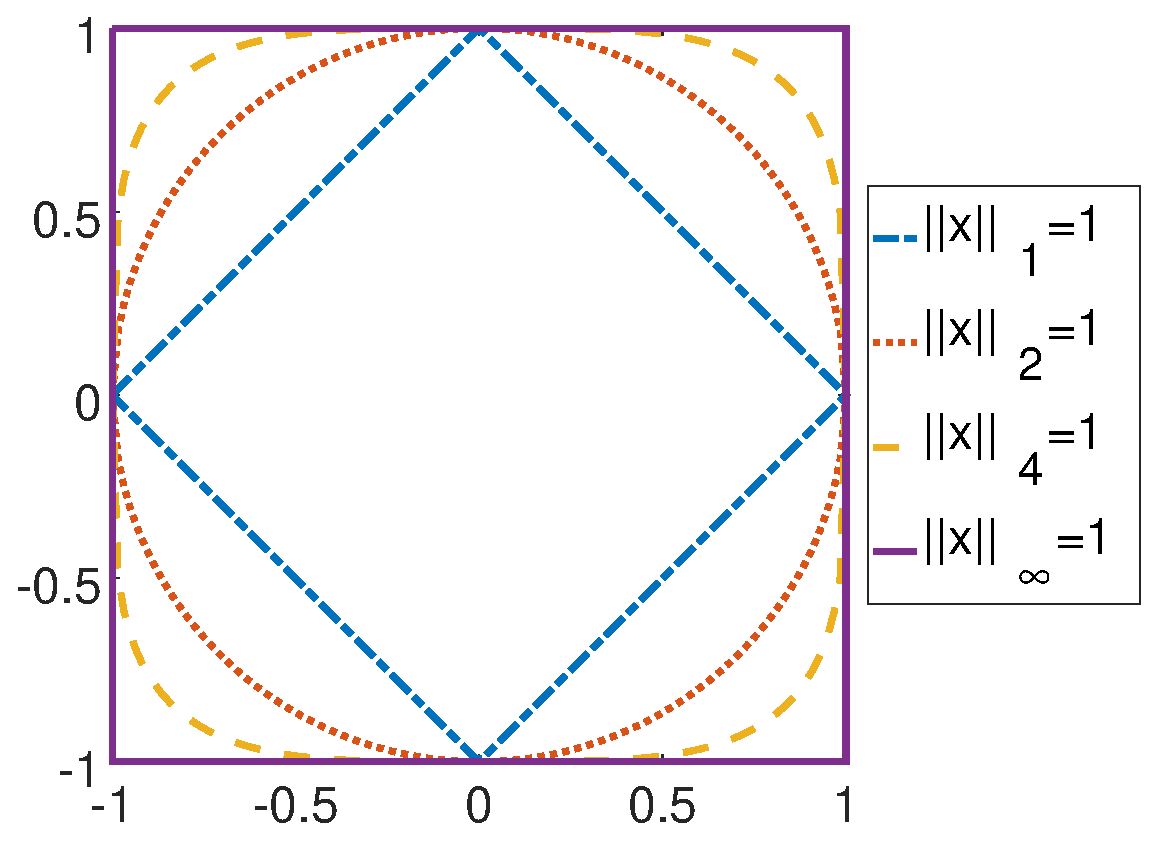
\includegraphics[width=0.45\textwidth]{chapters/notacao/pnormcode.eps}
     \caption{Curva de norma unitária.}
     \label{fig:curvaunit}
     \vspace{-30pt}
\end{wrapfigure}
Dado um vetor $\VECTOR{x} \in \mathbb{C}^{N}$,
é definida a norma $p$ de $\VECTOR{x}$  como $\|\VECTOR{x}\|_p$ \cite[pp. 33]{vetterli2014foundations}, 
\begin{equation}
\|\VECTOR{x}\|_p=\left(\sum_{n=1}^N |x_n|^p\right)^{\frac{1}{p}},
\end{equation}
em que $1 \leq p < \infty$; a norma $p$
também é denotada como norma $L_p$ ou ``$p$-norm'' em inglês.
Assim, dependendo do valor de $p$, entraremos em vários casos ou tipos de norma,
a Fig. \ref{fig:curvaunit} e os seguintes exemplos mostram alguns desses tipos.

\begin{example}[Norma taxicab - $p=1$:] Também chamada norma Manhattan
\begin{equation}
\|\VECTOR{x}\|_1=\sum_{n=1}^N |x_n|.
\end{equation}
\end{example}

\begin{example}[Norma euclidiana - $p=2$:] Também chamada norma euclidiana quadrada, 
a qual também pode ser representada como $\|\VECTOR{x}\|$; 
assim, ante a ausência de subíndice se entende que é a $2$-norm,
\begin{equation}
\|\VECTOR{x}\|_2\equiv \|\VECTOR{x}\| =\sqrt{\sum_{n=1}^N |x_n|^2}.
\end{equation}
Uma representação relativa à norma quadrada euclidiana é
\begin{equation}
\|\VECTOR{x}\|_2^2\equiv \|\VECTOR{x}\|^2=\sum_{n=1}^N |x_n|^2\equiv \VECTOR{x}^{*} \VECTOR{x},
\end{equation}
em que $\VECTOR{x}^{*}\equiv \VECTOR{\bar{x}}^{\transpose}$ 
representa a transposta do conjugado do vetor  $\VECTOR{x}$. 
\end{example}

\begin{example}[Norma com $p=\infty$:]
\begin{equation}
\|\VECTOR{x}\|_{\infty}=\max \left( |x_1|,~|x_2|,~...,~|x_n|,~...,~|x_N|\right)\equiv \max_n \left( |x_n|\right).
\end{equation}
\end{example}





%----------------------------------------------------------------------------------------
%	CHAPTER 1
%----------------------------------------------------------------------------------------
\chapterimage{chapter_head_2.pdf} % Chapter heading image

\chapter{Derivada de funções com variável vetorial}

%%%%%%%%%%%%%%%%%%%%%%%%%%%%%%%%%%%%%%%%%%%%%%%%%%%%%%%%%%%%%%%%%%%%%%%%%%%%%%%%%%%%%%%
%%%%%%%%%%%%%%%%%%%%%%%%%%%%%%%%%%%%%%%%%%%%%%%%%%%%%%%%%%%%%%%%%%%%%%%%%%%%%%%%%%%%%%%
\section{Derivada de $e(\mathbf{x})$ e $\mathbf{f}(\mathbf{x})$}

\begin{definition}\label{def:deltahor}
Se 
$\mathbf{x}\in \mathbb{R}^N$ é um vetor linha com elementos $x_n\in \mathbb{R}$ de modo que
$n\in \mathbb{N}$, $1 \leq n \leq N$, 
a função $e(\mathbf{x}): \mathbb{R}^N \rightarrow \mathbb{R}$ é um escalar, e
a função $\mathbf{f}(\mathbf{x}): \mathbb{R}^N \rightarrow \mathbb{R}^M$ é um vetor coluna, 
então definimos que:

\begin{equation}
\frac{\partial e(\mathbf{x}) }{\partial \mathbf{x}^{\transpose}}= 
\left[
\begin{matrix}
\frac{\partial e(\mathbf{x}) }{\partial x_{1}}&
\frac{\partial e(\mathbf{x}) }{\partial x_{2}}&
\hdots&
\frac{\partial e(\mathbf{x}) }{\partial x_{n}}&
\hdots&
\frac{\partial e(\mathbf{x}) }{\partial x_{N}}
\end{matrix}
\right]= {\bigcup\limits_{n=1}^{\rightarrow}}^{N}{\frac{\partial e(\mathbf{x}) }{\partial x_{n}}} 
\end{equation}

\begin{equation}
\frac{\partial \mathbf{f}(\mathbf{x}) }{\partial \mathbf{x}^{\transpose}}= 
\left[
\begin{matrix}
\frac{\partial \mathbf{f}(\mathbf{x}) }{\partial x_{1}}&
\frac{\partial \mathbf{f}(\mathbf{x}) }{\partial x_{2}}&
\hdots&
\frac{\partial \mathbf{f}(\mathbf{x}) }{\partial x_{n}}&
\hdots&
\frac{\partial \mathbf{f}(\mathbf{x}) }{\partial x_{N}}
\end{matrix}
\right]= {\bigcup\limits_{n=1}^{\rightarrow}}^{N}{\frac{\partial \mathbf{f}(\mathbf{x}) }{\partial x_{n}}} 
\end{equation}

\begin{equation}
\frac{\partial \mathbf{G}(\mathbf{x}) }{\partial \mathbf{x}^{\transpose}}= 
\left[
\begin{matrix}
\frac{\partial \mathbf{G}(\mathbf{x}) }{\partial x_{1}}&
\frac{\partial \mathbf{G}(\mathbf{x}) }{\partial x_{2}}&
\hdots&
\frac{\partial \mathbf{G}(\mathbf{x}) }{\partial x_{n}}&
\hdots&
\frac{\partial \mathbf{G}(\mathbf{x}) }{\partial x_{N}}
\end{matrix}
\right]= {\bigcup\limits_{n=1}^{\rightarrow}}^{N}{\frac{\partial \mathbf{G}(\mathbf{x}) }{\partial x_{n}}} 
\end{equation}
\end{definition}

\begin{definition}\label{def:deltaver}
Se 
$\mathbf{x}\in \mathbb{R}^N$ é um vetor coluna com elementos $x_n\in \mathbb{R}$ de modo que
$n\in \mathbb{N}$, $1 \leq n \leq N$, 
a função $e(\mathbf{x}): \mathbb{R}^N \rightarrow \mathbb{R}$ é um escalar, e
a função $\mathbf{f}(\mathbf{x}): \mathbb{R}^N \rightarrow \mathbb{R}^M$ é um vetor coluna, 
então definimos que:
\begin{equation}
\frac{\partial e(\mathbf{x}) }{\partial \mathbf{x}}= 
\left[
\begin{matrix}
\frac{\partial e(\mathbf{x}) }{\partial x_{1}} \\
\frac{\partial e(\mathbf{x}) }{\partial x_{2}} \\
\vdots \\
\frac{\partial e(\mathbf{x}) }{\partial x_{n}} \\
\vdots \\
\frac{\partial e(\mathbf{x}) }{\partial x_{N}} 
\end{matrix}
\right] = \functrans \left( \frac{\partial e(\mathbf{x}) }{\partial \mathbf{x}^{\transpose}} \right) =
\funcvec \left( \frac{\partial e(\mathbf{x}) }{\partial \mathbf{x}^{\transpose}} \right) =
{\bigcup\limits_{n=1}^{\downarrow}}^{N}{\frac{\partial e(\mathbf{x}) }{\partial x_{n}}} 
\end{equation}

\begin{equation}
\frac{\partial \mathbf{f}(\mathbf{x}) }{\partial \mathbf{x}}= 
\left[
\begin{matrix}
\frac{\partial \mathbf{f}(\mathbf{x}) }{\partial x_{1}} \\
\frac{\partial \mathbf{f}(\mathbf{x}) }{\partial x_{2}} \\
\vdots \\
\frac{\partial \mathbf{f}(\mathbf{x}) }{\partial x_{n}} \\
\vdots \\
\frac{\partial \mathbf{f}(\mathbf{x}) }{\partial x_{N}}
\end{matrix}
\right] =  \funcvec \left( \frac{\partial \mathbf{f}(\mathbf{x}) }{\partial \mathbf{x}^{\transpose}} \right) =
{\bigcup\limits_{n=1}^{\downarrow}}^{N}{\frac{\partial \mathbf{f}(\mathbf{x}) }{\partial x_{n}}}
\end{equation}

\begin{equation}
\frac{\partial \mathbf{G}(\mathbf{x}) }{\partial \mathbf{x}}= 
\left[
\begin{matrix}
\frac{\partial \mathbf{G}(\mathbf{x}) }{\partial x_{1}} \\
\frac{\partial \mathbf{G}(\mathbf{x}) }{\partial x_{2}} \\
\vdots \\
\frac{\partial \mathbf{G}(\mathbf{x}) }{\partial x_{n}} \\
\vdots \\
\frac{\partial \mathbf{G}(\mathbf{x}) }{\partial x_{N}}
\end{matrix}
\right] = {\bigcup\limits_{n=1}^{\downarrow}}^{N}{\frac{\partial \mathbf{G}(\mathbf{x}) }{\partial x_{n}}}
\end{equation}
\end{definition}
%%%%%%%%%%%%%%%%%%%%%%%%%%%%%%%%%%%%%%%%%%%%%%%%%%%%%%%%%%%%%%%%%%%%%%%%%%%%%%%%%%%%%%%
%%%%%%%%%%%%%%%%%%%%%%%%%%%%%%%%%%%%%%%%%%%%%%%%%%%%%%%%%%%%%%%%%%%%%%%%%%%%%%%%%%%%%%%
\section{Derivada de $\mathbf{A}\mathbf{x}$}

\begin{theorem}\label{theo:derAx}
Se 
$\mathbf{x}\in \mathbb{R}^N$ é um vetor coluna com elementos $x_n$ de modo que
$n\in \mathbb{N}$, $1 \leq n \leq N$, e 
$\mathbf{A} \in \mathbb{R}^{M\times N}$ é uma matriz com elementos $a_{mn}$ de modo que
$m\in \mathbb{N}$, $1 \leq m \leq M$, então se cumpre que:
\begin{equation}
\frac{\partial \mathbf{A}\mathbf{x}}{\partial x_n}=a_{:n}
\end{equation}
A demostração pode ser vista na Prova \ref{proof:theo:derAx}.
\end{theorem}

\begin{corollaryT}[Derivada de $\mathbf{A}\mathbf{x}$ em relação ao vector $\mathbf{x}^{\transpose}$]\label{coro:derAx1}
Aplicando a Definição \ref{def:deltahor} junto ao Teorema \ref{theo:derAx}, é
fácil deduzir que:
\begin{equation}
\frac{\partial \mathbf{A}\mathbf{x}}{\partial \mathbf{x}^{\transpose}}=
\left[
\begin{matrix}
 a_{:1} &  a_{:2} &  \cdots &  a_{:N}
\end{matrix}
\right]=
\mathbf{A}
\end{equation}
\end{corollaryT}

\begin{corollaryT}[Derivada de $\mathbf{A}\mathbf{x}$ em relação ao vector $\mathbf{x}$]\label{coro:derAx2}
Aplicando a Definição \ref{def:deltaver} junto ao Teorema \ref{theo:derAx}, é
fácil deduzir que:
\begin{equation}
\frac{\partial \mathbf{A}\mathbf{x}}{\partial \mathbf{x}}=
\left[
\begin{matrix}
 a_{:1} \\  a_{:2} \\  \vdots \\  a_{:N}
\end{matrix}
\right]=\funcvec(\mathbf{A})
\end{equation}
\end{corollaryT}

\begin{corollaryT}[Derivada de $\mathbf{a}^{\transpose}\mathbf{x}$ em relação ao vector $\mathbf{x}^{\transpose}$]\label{coro:derAx3}
Aplicando a Definição \ref{def:deltahor} junto ao Teorema \ref{theo:derAx} e sabendo que $\mathbf{a}^{\transpose}$
é um vetor linha, é
fácil deduzir que:
\begin{equation}
\frac{\partial \mathbf{a}^{\transpose}\mathbf{x}}{\partial \mathbf{x}^{\transpose}}=\mathbf{a}^{\transpose}
\end{equation}
\end{corollaryT}

\begin{corollaryT}[Derivada de $\mathbf{a}^{\transpose}\mathbf{x}$ em relação ao vector $\mathbf{x}$]\label{coro:derAx4}
Aplicando a Definição \ref{def:deltaver} junto ao Teorema \ref{theo:derAx} e sabendo que $\mathbf{a}^{\transpose}$
é um vetor linha, é
fácil deduzir que:
\begin{equation}
\frac{\partial \mathbf{a}^{\transpose}\mathbf{x}}{\partial \mathbf{x}}=\mathbf{a}
\end{equation}
\end{corollaryT}

%%%%%%%%%%%%%%%%%%%%%%%%%%%%%%%%%%%%%%%%%%%%%%%%%%%%%%%%%%%%%%%%%%%%%%%%%%%%%%%%%%%%%%%
%%%%%%%%%%%%%%%%%%%%%%%%%%%%%%%%%%%%%%%%%%%%%%%%%%%%%%%%%%%%%%%%%%%%%%%%%%%%%%%%%%%%%%%
\section{Derivada de $||\mathbf{A}\mathbf{x}||^2$ 
}

\begin{theorem}\label{theo:derxAtAx}
Se 
$\mathbf{x}\in \mathbb{R}^N$ é um vetor coluna com elementos $x_n$ de modo que
$n\in \mathbb{N}$, $1 \leq n \leq N$, e 
$\mathbf{A} \in \mathbb{R}^{M\times N}$ é uma matriz com elementos $a_{mn}$ de modo que
$m\in \mathbb{N}$, $1 \leq m \leq M$, então se cumpre que:
\begin{equation}
\begin{matrix}
\frac{\partial ||\mathbf{A}\mathbf{x}||^2 }{\partial x_n}&=&
\frac{\partial \left(\mathbf{A}\mathbf{x}\right)^{\transpose}\left(\mathbf{A}\mathbf{x}\right)}{\partial x_n}&=&
2\left(\mathbf{A}\mathbf{x}\right)^{\transpose}a_{:n}\\
~&~&~&=& 2\left(a_{:n}\right)^{\transpose}\mathbf{A}\mathbf{x}
\end{matrix}
\end{equation}
A demostração pode ser vista na Prova \ref{proof:theo:derxAtAx}.
\end{theorem}

\begin{corollaryT}[Derivada de $||\mathbf{A}\mathbf{x}||^2$ em relação ao vector $\mathbf{x}^{\transpose}$]\label{coro:derxAtAx1}
Aplicando a Definição \ref{def:deltahor} junto ao Teorema \ref{theo:derxAtAx}, é
fácil deduzir que:
\begin{equation}
\frac{\partial ||\mathbf{A}\mathbf{x}||^2 }{\partial \mathbf{x}^{\transpose}}=
\frac{\partial \left(\mathbf{A}\mathbf{x}\right)^{\transpose}\left(\mathbf{A}\mathbf{x}\right)}{\partial \mathbf{x}^{\transpose}}=
2\left(\mathbf{A}^{\transpose}\mathbf{A}\mathbf{x}\right)^{\transpose}
\end{equation}
\end{corollaryT}

\begin{corollaryT}[Derivada de $||\mathbf{A}\mathbf{x}||^2$ em relação ao vector $\mathbf{x}$]\label{coro:derxAtAx2}
Aplicando a Definição \ref{def:deltaver} junto ao Teorema \ref{theo:derxAtAx}, é
fácil deduzir que:
\begin{equation}
\frac{\partial ||\mathbf{A}\mathbf{x}||^2 }{\partial \mathbf{x}}=
\frac{\partial \left(\mathbf{A}\mathbf{x}\right)^{\transpose}\left(\mathbf{A}\mathbf{x}\right)}{\partial \mathbf{x}}=
2 \mathbf{A}^{\transpose}\mathbf{A}\mathbf{x}
\end{equation}
\end{corollaryT}

%%%%%%%%%%%%%%%%%%%%%%%%%%%%%%%%%%%%%%%%%%%%%%%%%%%%%%%%%%%%%%%%%%%%%%%%%%%%%%%%%%%%%%%
%%%%%%%%%%%%%%%%%%%%%%%%%%%%%%%%%%%%%%%%%%%%%%%%%%%%%%%%%%%%%%%%%%%%%%%%%%%%%%%%%%%%%%%
\section{Derivada de $||\mathbf{A}\mathbf{x}-\mathbf{b}||_{\mathbf{C}}^2$ 
}

\begin{theorem}\label{theo:derAxbAxb}
Se 
$\mathbf{x}\in \mathbb{R}^N$ é um vetor coluna com elementos $x_n$ de modo que
$n\in \mathbb{N}$, $1 \leq n \leq N$, 
$\mathbf{b}\in \mathbb{R}^M$ é um vetor coluna com elementos $b_m$ de modo que
$m\in \mathbb{N}$, $1 \leq m \leq M$,  
$\mathbf{A} \in \mathbb{R}^{M\times N}$ é uma matriz com elementos $a_{mn}$, e
$\mathbf{C} \in \mathbb{R}^{M\times M}$ é uma matriz diagonal, 
então se cumpre que:
\begin{equation}
\begin{matrix}
\frac{\partial ||\mathbf{A}\mathbf{x}-\mathbf{b}||_{\mathbf{C}}^2}{\partial x_n}&=&
\frac{\partial \left(\mathbf{A}\mathbf{x}-\mathbf{b}\right)^{\transpose}\mathbf{C}\left(\mathbf{A}\mathbf{x}-\mathbf{b}\right)}{\partial x_n}&=&
2\left(\mathbf{A}\mathbf{x}-\mathbf{b}\right)^{\transpose}\mathbf{C}a_{:n}\\
~&~&~&=& 2\left(a_{:n}\right)^{\transpose}\mathbf{C}\left(\mathbf{A}\mathbf{x}-  \mathbf{b}\right)
\end{matrix}
\end{equation}
A demostração pode ser vista na Prova \ref{proof:theo:derAxbAxb}.
\end{theorem}

\begin{corollaryT}[Derivada de $||\mathbf{A}\mathbf{x}-\mathbf{b}||_{\mathbf{C}}^2$ em relação ao vector $\mathbf{x}^{\transpose}$]\label{coro:derAxbAxb1}
Aplicando a Definição \ref{def:deltahor} junto ao Teorema \ref{theo:derAxbAxb}, é
fácil deduzir que:
\begin{equation}
\frac{\partial ||\mathbf{A}\mathbf{x}-\mathbf{b}||^2}{\partial \mathbf{x}^{\transpose}}=
2\left(\mathbf{A}\mathbf{x}- \mathbf{b} \right)^{\transpose}\mathbf{C}\mathbf{A}
\end{equation}
\end{corollaryT}

\begin{corollaryT}[Derivada de $||\mathbf{A}\mathbf{x}-\mathbf{b}||_{\mathbf{C}}^2$ em relação ao vector $\mathbf{x}$]\label{coro:derAxbAxb2}
Aplicando a Definição \ref{def:deltaver} junto ao Teorema \ref{theo:derAxbAxb}, é
fácil deduzir que:
\begin{equation}
\frac{\partial ||\mathbf{A}\mathbf{x}-\mathbf{b}||^2}{\partial \mathbf{x} }=
2 \mathbf{A}^{\transpose}\mathbf{C}\left(\mathbf{A}\mathbf{x}-\mathbf{b}\right)
\end{equation}
\end{corollaryT}

%%%%%%%%%%%%%%%%%%%%%%%%%%%%%%%%%%%%%%%%%%%%%%%%%%%%%%%%%%%%%%%%%%%%%%%%%%%%%%%%%%%%%%%
%%%%%%%%%%%%%%%%%%%%%%%%%%%%%%%%%%%%%%%%%%%%%%%%%%%%%%%%%%%%%%%%%%%%%%%%%%%%%%%%%%%%%%%
\section{Derivada de $||\mathbf{f}(\mathbf{x})-\mathbf{b}||_{\mathbf{C}}^2$  
(Aproximação e exato)
}

\begin{theorem}[Valor exato]\label{theo:derfxbCfxb0}
Se 
$\mathbf{x}\in \mathbb{R}^N$ é um vetor coluna, 
$\mathbf{b}\in \mathbb{R}^M$ é um vetor coluna,  
$\mathbf{f}: \mathbb{R}^{N}\rightarrow \mathbb{R}^{M}$ é uma função de valor vectorial, e
$\mathbf{C} \in \mathbb{R}^{M\times M}$ é uma matriz diagonal, 
então se cumpre que:
\begin{equation}
\frac{\partial ||\mathbf{f}(\mathbf{x})-\mathbf{b}||_{\mathbf{C}}^2}{\partial \mathbf{x}} =
2 \mathbf{J}(\mathbf{x})^{\transpose}\mathbf{C}\left[\mathbf{f}(\mathbf{x})-\mathbf{b}\right],
\end{equation}
onde $\mathbf{J}(\mathbf{x})$ é a matriz Jacobiana de $\mathbf{f}(\mathbf{x})$.

A demostração pode ser vista na Prova \ref{proof:theo:derfxbCfxb0}.
\end{theorem}
\index{Jacobian}
\index{Serie de Taylor}

\begin{theorem}[Valor aproximado]\label{theo:derfxbCfxb}
Se 
$\mathbf{x}\in \mathbb{R}^N$ é um vetor coluna, 
$\mathbf{b}\in \mathbb{R}^M$ é um vetor coluna,  
$\mathbf{f}: \mathbb{R}^{N}\rightarrow \mathbb{R}^{M}$ é uma função de valor vectorial, e
$\mathbf{C} \in \mathbb{R}^{M\times M}$ é uma matriz diagonal, 
então se cumpre que:
\begin{equation}
\frac{\partial ||\mathbf{f}(\mathbf{x})-\mathbf{b}||_{\mathbf{C}}^2}{\partial \mathbf{x}} \approx
2 \mathbf{J}(\mathbf{p})^{\transpose}\mathbf{C}\left[\mathbf{J}(\mathbf{p})\left(\mathbf{x} - \mathbf{p}\right)-\left(\mathbf{b}-\mathbf{f}(\mathbf{p})\right)\right]
\end{equation}

Onde é considerada a aproximação
$\mathbf{f}(\mathbf{x})\approx \mathbf{f}(\mathbf{p})+\mathbf{J}(\mathbf{p})\left(\mathbf{x}-\mathbf{p}\right)$,
usando a serie de Taylor para funções multivariáveis. Sendo $\mathbf{p}$ um ponto fixo no domínio de $\mathbf{f}(\mathbf{x})$,  ao redor do qual é feita  aproximação
da função $\mathbf{f}(\mathbf{x})$,
e $\mathbf{J}(\mathbf{p})$ é a matriz Jacobiana de $\mathbf{f}(\mathbf{x})$ avaliado no ponto $\mathbf{p}$.

A demostração pode ser vista na Prova \ref{proof:theo:derfxbCfxb}.
\end{theorem}
\index{Jacobian}
\index{Serie de Taylor}

%%%%%%%%%%%%%%%%%%%%%%%%%%%%%%%%%%%%%%%%%%%%%%%%%%%%%%%%%%%%%%%%%%%%%%%%%%%%%%%%%%%%%%%
%%%%%%%%%%%%%%%%%%%%%%%%%%%%%%%%%%%%%%%%%%%%%%%%%%%%%%%%%%%%%%%%%%%%%%%%%%%%%%%%%%%%%%%
\section{Derivada de segundo ordem de $||\mathbf{f}(\mathbf{x})-\mathbf{b}||_{\mathbf{C}}^2$  
(Aproximação)
}

\begin{theorem}[Valor exato]\label{theo:der2fxbCfxb0}
Se 
$\mathbf{x}\in \mathbb{R}^N$ é um vetor coluna, 
$\mathbf{b}\in \mathbb{R}^M$ é um vetor coluna,  
$\mathbf{f}: \mathbb{R}^{N}\rightarrow \mathbb{R}^{M}$ é uma função de valor vectorial,
$\mathbf{C} \in \mathbb{R}^{M\times M}$ é uma matriz diagonal, e
definida a função $e(\mathbf{x})$,
\begin{equation}
e(\mathbf{x})= ||\mathbf{f}(\mathbf{x})-\mathbf{b}||_{\mathbf{C}}^2.
\end{equation}
Então a matriz Hessiana $\mathbf{H}(\mathbf{x})$ de $e(\mathbf{x})$ é igual a:
\begin{equation}
\mathbf{H}(\mathbf{x}) = \frac{\partial}{\partial \mathbf{x}^{\transpose}}\left(  
\frac{\partial e(\mathbf{x}) }{\partial \mathbf{x}} \right) = 2 
\mathbf{B}_{H}(\mathbf{x}) \mathbf{B}_{D}(\mathbf{x})
+2 \mathbf{J}(\mathbf{x})^{\transpose}\mathbf{C} \mathbf{J}(\mathbf{x}),
\end{equation}
onde 
\begin{equation}
 \mathbf{B}_{H}(\mathbf{x})={\bigcup\limits_{n=1}^{\rightarrow}}^{N}\left\{\frac{\partial \mathbf{J}(\mathbf{x})^{\transpose} }{\partial x_{n}}\right\},
\end{equation}
\begin{equation}
 \mathbf{B}_{D}(\mathbf{x})={\bigcup\limits_{n=1}^{\searrow}}^{N}\left\{ \mathbf{C} \left( \mathbf{f}(\mathbf{x})-\mathbf{b} \right) \right\}. 
\end{equation}

A demostração pode ser vista na Prova \ref{proof:theo:der2fxbCfxb0}.
\end{theorem}

\begin{theorem}[Valor aproximado]\label{theo:der2fxbCfxb}
Se 
$\mathbf{x}\in \mathbb{R}^N$ é um vetor coluna, 
$\mathbf{b}\in \mathbb{R}^M$ é um vetor coluna,  
$\mathbf{f}: \mathbb{R}^{N}\rightarrow \mathbb{R}^{M}$ é uma função de valor vectorial,
$\mathbf{C} \in \mathbb{R}^{M\times M}$ é uma matriz diagonal, e
definida a função $e(\mathbf{x})$,
\begin{equation}
e(\mathbf{x})= ||\mathbf{f}(\mathbf{x})-\mathbf{b}||_{\mathbf{C}}^2.
\end{equation}
Então a matriz Hessiana de $e(\mathbf{x})$ é igual a:
\begin{equation}
\frac{\partial}{\partial \mathbf{x}^{\transpose}}\left(  
\frac{\partial e(\mathbf{x}) }{\partial \mathbf{x}} \right) \approx
2 \mathbf{J}(\mathbf{p})^{\transpose}\mathbf{C} \mathbf{J}(\mathbf{p})
\end{equation}

Onde é considerada a aproximação
$\mathbf{f}(\mathbf{x})\approx \mathbf{f}(\mathbf{p})+\mathbf{J}(\mathbf{p})\left(\mathbf{x}-\mathbf{p}\right)$,
usando a serie de Taylor para funções multivariáveis. Sendo $\mathbf{p}$ um ponto fixo no domínio de $\mathbf{f}(\mathbf{x})$,  ao redor do qual é feita  aproximação
da função $\mathbf{f}(\mathbf{x})$,
e $\mathbf{J}(\mathbf{p})$ é a matriz Jacobiana de $\mathbf{f}(\mathbf{x})$ avaliado no ponto $\mathbf{p}$.

A demostração pode ser vista na Prova \ref{proof:theo:der2fxbCfxb}.
\end{theorem}
\index{Hessian}
\index{Serie de Taylor}


%%%%%%%%%%%%%%%%%%%%%%%%%%%%%%%%%%%%%%%%%%%%%%%%%%%%%%%%%%%%%%%%%%%%%%%%%%%%%%%%%%%%%%%
%%%%%%%%%%%%%%%%%%%%%%%%%%%%%%%%%%%%%%%%%%%%%%%%%%%%%%%%%%%%%%%%%%%%%%%%%%%%%%%%%%%%%%%
\section{Derivada de $||\mathbf{f}(\mathbf{x})-\mathbf{b}||_{\mathbf{C}}^2+\alpha||\mathbf{x}-\mathbf{q}||_{\mathbf{D}}^2$  
(Aproximação)
}

\begin{theorem}\label{theo:derfxbCfxbxqDxq}
Se 
$\mathbf{x}\in \mathbb{R}^N$ é um vetor coluna, 
$\mathbf{b}\in \mathbb{R}^M$ é um vetor coluna,
$\mathbf{q}\in \mathbb{R}^N$ é um vetor coluna, 
$\mathbf{f}: \mathbb{R}^{N}\rightarrow \mathbb{R}^{M}$ é uma função de valor vectorial, 
$\mathbf{C} \in \mathbb{R}^{M\times M}$ é uma matriz diagonal, e
$\mathbf{D} \in \mathbb{R}^{N\times N}$ é uma matriz diagonal, 
então se cumpre que:
\begin{equation}
\frac{\partial \left(||\mathbf{f}(\mathbf{x})-\mathbf{b}||_{\mathbf{C}}^2+\alpha||\mathbf{x}-\mathbf{q}||_{\mathbf{D}}^2\right)}{\partial \mathbf{x}} \approx
2 \mathbf{J}(\mathbf{p})^{\transpose}\mathbf{C}\left[\mathbf{J}(\mathbf{p})\mathbf{x} - \mathbf{J}(\mathbf{p})\mathbf{p}-\mathbf{b}+\mathbf{f}(\mathbf{p})\right]
+2\alpha\mathbf{D}\left(\mathbf{x}-\mathbf{q}\right)
\end{equation}

Onde é considerada a aproximação
$\mathbf{f}(\mathbf{x})\approx \mathbf{f}(\mathbf{p})+\mathbf{J}(\mathbf{p})\left(\mathbf{x}-\mathbf{p}\right)$,
usando a serie de Taylor para funções multivariáveis. Sendo $\mathbf{p}$ um ponto fixo no domínio de $\mathbf{f}(\mathbf{x})$,  ao redor do qual é feita  aproximação
da função $\mathbf{f}(\mathbf{x})$,
e $\mathbf{J}(\mathbf{p})$ é a matriz Jacobiana de $\mathbf{f}(\mathbf{x})$ avaliado no ponto $\mathbf{p}$.

A demostração pode ser vista na Prova \ref{proof:theo:derfxbCfxbxqDxq}.
\end{theorem}

\index{Serie de Taylor}
%----------------------------------------------------------------------------------------
%	CHAPTER 2
%----------------------------------------------------------------------------------------
\chapterimage{chapter_head_2.pdf} % Chapter heading image

\chapter{Minimização de funções com variável vetorial}

\begin{remark}
Palavras chave: 
Pseudo-inversa de Moore-Penrose,
regularização de Tikhonov,
problema inverso, 
minimização do erro quadrático. 
\end{remark}
%%%%%%%%%%%%%%%%%%%%%%%%%%%%%%%%%%%%%%%%%%%%%%%%%%%%%%%%%%%%%%%%%%%%%%%%%%%%%%%%%%%%%%%
\section{Minimização de $||\mathbf{A}\mathbf{x}-\mathbf{b}||_{\mathbf{C}}^2$
}

\begin{theorem}\label{theo:minAxbCAxb}
Dados,
um vetor coluna $\mathbf{x}\in \mathbb{R}^N$, 
um vetor coluna $\mathbf{b}\in \mathbb{R}^M$,  
uma matriz $\mathbf{A} \in \mathbb{R}^{M\times N}$, 
uma matriz diagonal $\mathbf{C} \in \mathbb{R}^{M\times M}$, e 
definida a Eq. (\ref{eq:minAxbCAxb1}),
\begin{equation}\label{eq:minAxbCAxb1}
e(\mathbf{x})=||\mathbf{A}\mathbf{x}-\mathbf{b}||_{\mathbf{C}}^2.
\end{equation}
Se desejamos ter o valor $\mathbf{\hat{x}}$ que minimiza o escalar $e(\mathbf{\hat{x}})$,
devemos usar a Eq. (\ref{eq:minAxbCAxb2}),
\begin{equation}\label{eq:minAxbCAxb2}
\mathbf{\hat{x}} =
\left[ \mathbf{A}^{\transpose}\mathbf{C} \mathbf{A} \right]^{-1}\mathbf{A}^{\transpose}\mathbf{C}\mathbf{b}.
\end{equation}
Assim, o mínimo existe só sim $\mathbf{A}^{\transpose}\mathbf{C} \mathbf{A}$ tem inversa.

A demostração pode ser vista na Prova \ref{proof:theo:minAxbCAxb}.
\end{theorem}

\index{Pseudo-inversa de Moore-Penrose}
\index{Problema inverso!Linear}
\index{Minimização do erro quadrático!Linear}


%%%%%%%%%%%%%%%%%%%%%%%%%%%%%%%%%%%%%%%%%%%%%%%%%%%%%%%%%%%%%%%%%%%%%%%%%%%%%%%%%%%%%%%
\section{Minimização de $||\mathbf{f}(\mathbf{x})-\mathbf{b}||_{\mathbf{C}}^2$
(solução iterativa)
}

\begin{theorem}\label{theo:minfxbCfxb}
Dados,
um vetor coluna $\mathbf{x}\in \mathbb{R}^N$, 
um vetor coluna $\mathbf{b}\in \mathbb{R}^M$,  
uma função $\mathbf{f}:\mathbb{R}^{N} \rightarrow \mathbb{R}^{M}$, 
uma matriz diagonal $\mathbf{C} \in \mathbb{R}^{M\times M}$, e 
definida a Eq. (\ref{eq:minfxbCfxb1}),
\begin{equation}\label{eq:minfxbCfxb1}
e(\mathbf{\hat{x}})=||\mathbf{f}(\mathbf{x})-\mathbf{b}||_{\mathbf{C}}^2.
\end{equation}
Se desejamos ter o valor $\mathbf{\hat{x}}$ que minimiza o escalar $e(\mathbf{\hat{x}})$,
este valor pode ser achado usando iterativamente a Eq. (\ref{eq:minfxbCfxb2}),
\begin{equation}\label{eq:minfxbCfxb2}
\mathbf{\hat{x}}_{k+1} \leftarrow \mathbf{\hat{x}}_k+
\left[ \mathbf{J}(\mathbf{\hat{x}}_k)^{\transpose}\mathbf{C} \mathbf{J}(\mathbf{\hat{x}}_k) \right]^{-1}
 \mathbf{J}(\mathbf{\hat{x}}_k)^{\transpose}\mathbf{C}\left[\mathbf{b}-\mathbf{f}(\mathbf{\hat{x}}_k)\right]
\end{equation}
Onde  $\mathbf{J}(\mathbf{x})$ é a matriz Jacobiana de $\mathbf{f}(\mathbf{x})$.
A busca iterativa é considerada falida quando 
$\mathbf{J}(\mathbf{\hat{x}}_k)^{\transpose}$ $\mathbf{C}$ $\mathbf{J}(\mathbf{\hat{x}}_k)$
não tem inversa.

A demostração pode ser vista na Prova \ref{proof:theo:minfxbCfxb}.
\end{theorem}

\index{Regularização! Regularização de Tikhonov}
\index{Problema inverso!Não linear}
\index{Minimização do erro quadrático!Não linear}

%%%%%%%%%%%%%%%%%%%%%%%%%%%%%%%%%%%%%%%%%%%%%%%%%%%%%%%%%%%%%%%%%%%%%%%%%%%%%%%%%%%%%%%
\section{Minimização de $||\mathbf{f}(\mathbf{x})-\mathbf{b}||_{\mathbf{C}}^2+\alpha||\mathbf{x}||_{\mathbf{D}}^2$  
(solução iterativa)
}

\begin{theorem}\label{theo:minfxbCfxbaxax}
Sabendo que, $\mathbf{x}$ é um vetor com $N$ elementos, $\mathbf{f}(\mathbf{x})$ e 
$\mathbf{b}$ são vetores coluna de $M$ elementos sendo $\mathbf{b}$ uma constante,
$\mathbf{C}$ uma matriz diagonal de $M \times M$ e 
$\mathbf{D}$ uma matriz diagonal de $N \times N$ :
Se desejamos minimizar o valor de $E$, visto na Eq. (\ref{eq:minfxbCfxb1}), em relação a $\mathbf{x}$.
\begin{equation}\label{eq:minfxbCfxbaxax1}
E=||\mathbf{f}(\mathbf{x})-\mathbf{b}||_{\mathbf{C}}^2+\alpha||\mathbf{x}||_{\mathbf{D}}^2
\end{equation}

\begin{equation}
\mathbf{x}_{k+1}\approx \mathbf{x}_k+
\left[ \mathbf{J}(\mathbf{x}_k)^{\transpose}\mathbf{C} \mathbf{J}(\mathbf{x}_k) +\alpha\mathbf{D} \right]^{-1}
 \left[\mathbf{J}(\mathbf{x}_k)^{\transpose}\mathbf{C}\left(\mathbf{b}-\mathbf{f}(\mathbf{x}_k)\right)-\alpha\mathbf{D}\mathbf{x}\right]
\end{equation}
Onde  $\mathbf{J}(\mathbf{x})$ é a matriz Jacobiana de $\mathbf{f}(\mathbf{x})$.
\end{theorem} 

\index{Regularização! Regularização de Tikhonov}
\index{Problema inverso!Não linear}
\index{Minimização do erro quadrático}


%%%%%%%%%%%%%%%%%%%%%%%%%%%%%%%%%%%%%%%%%%%%%%%%%%%%%%%%%%%%%%%%%%%%%%%%%%%%%%%%%%%%%%%
\section{Minimização de $||\mathbf{f}(\mathbf{x})-\mathbf{b}||_{\mathbf{C}}^2+\alpha||\mathbf{x}-\mathbf{q}||_{\mathbf{D}}^2$  
(solução iterativa)
}


%%%%%%%%%%%%%%%%%%%%%%%%%%%%%%%%%%%%%%%%%%%%%%%%%%%%%%%%%%%%%%%%%%%%%%%%%%%%%%%%%%%%%%%
\section{Minimização de $\frac{||\mathbf{f}(\mathbf{x})-\mathbf{b}||^2}{||\mathbf{b}||^2}$
$+\alpha\frac{||\mathbf{x}-\mathbf{q}||^2}{||\mathbf{q}||^2}$  
(solução iterativa)
}

\textcolor{red}{Inventado por mi ..., creo.}

%%%%%%%%%%%%%%%%%%%%%%%%%%%%%%%%%%%%%%%%%%%%%%%%%%%%%%%%%%%%%%%%%%%%%%%%%%%%%%%%%%%%%%%
\section{Minimização de $||\mathbf{f}(\mathbf{x})-\mathbf{b}||_{\mathbf{B}^{-2}}^2$
$+\alpha||\mathbf{x}-\mathbf{q}||_{\mathbf{Q}^{-2}}^2$  
(solução iterativa)
}


\textcolor{red}{Inventado por mi ..., creo Nenhun valor de $\mathbf{b}$ ou $\mathbf{q}$ pode ser zero.}




%----------------------------------------------------------------------------------------
%	PART
%----------------------------------------------------------------------------------------
\part{Part Two}

%----------------------------------------------------------------------------------------
%	CHAPTER 2
%----------------------------------------------------------------------------------------

\chapterimage{chapter_head_1.pdf} % Chapter heading image
\chapter{Examples 1}\index{Examples}




\begin{remark}
\lipsum[2]
\end{remark}




%----------------------------------------------------------------------------------------
%	CHAPTER 3
%----------------------------------------------------------------------------------------

\chapterimage{chapter_head_1.pdf} % Chapter heading image
\chapter{Examples 2}\index{Examples}

This is an example of examples.

\begin{example}[Example name]
\lipsum[2]
\begin{equation}
f(x)
\end{equation}
\end{example}


\begin{exercise}
\lipsum[2]
\end{exercise}


\begin{problem}
\lipsum[2]
\end{problem}

\begin{figure}[h]
\centering
\includegraphics[scale=0.5]{placeholder}
\caption{Figure caption}
\end{figure}


%----------------------------------------------------------------------------------------
%	CHAPTER 4
%----------------------------------------------------------------------------------------

\chapterimage{chapter_head_1.pdf} % Chapter heading image
\chapter{Examples 3}\index{Examples}



\begin{theorem}[Name of the theorem]
\lipsum[2]
\begin{equation}
f(x)
\end{equation}
\end{theorem}


\begin{theorem}
\lipsum[2]
\end{theorem}

\begin{definition}[Definition name]
\lipsum[2]
\end{definition}

\begin{corollary}[Corollary name]
\lipsum[2]
\end{corollary}

\begin{proposition}[Proposition name]
\lipsum[2]
\begin{equation}
f(x)
\end{equation}
\end{proposition}

\begin{proposition} 
\lipsum[2]
\end{proposition}



%----------------------------------------------------------------------------------------
%	BIBLIOGRAPHY
%----------------------------------------------------------------------------------------

\chapter*{Bibliography}
\addcontentsline{toc}{chapter}{\textcolor{ocre}{Bibliography}}
\section*{Books}
\addcontentsline{toc}{section}{Books}
\printbibliography[heading=bibempty,type=book]
\section*{Articles}
\addcontentsline{toc}{section}{Articles}
\printbibliography[heading=bibempty,type=article]

%----------------------------------------------------------------------------------------
%	INDEX
%----------------------------------------------------------------------------------------

\cleardoublepage
\phantomsection
\setlength{\columnsep}{0.75cm}
\addcontentsline{toc}{chapter}{\textcolor{ocre}{Index}}
\printindex

%----------------------------------------------------------------------------------------

\end{document}
